%=============================================================
%  TRABAJO FIN DE GRADO
%  Determinantes del gasto en seguros sanitarios privados
%  en España: tiempos de espera, renta y comportamiento
%  diferido (2016-2024)
%
%  Universidad de Murcia · Grado en Economía · 2025-2026
%=============================================================

% Para compilación rápida en Overleaf free, descomentar 'draft':
% \documentclass[12pt, a4paper, twoside, draft]{report}
\documentclass[12pt, a4paper, twoside]{report}

%-------------------------------------------------------------
% OPTIMIZACIÓN: Filtrar warnings de Overfull/Underfull
%-------------------------------------------------------------
\usepackage{silence}
\WarningFilter{latex}{Overfull}
\WarningFilter{latex}{Underfull}

%-------------------------------------------------------------
% CODIFICACIÓN E IDIOMA
%-------------------------------------------------------------
\usepackage[utf8]{inputenc}
\usepackage[T1]{fontenc}
\usepackage[spanish, es-nodecimaldot]{babel}

%-------------------------------------------------------------
% TIPOGRAFÍA
%-------------------------------------------------------------
\usepackage{lmodern}           % Latin Modern (mejora cm estándar)
% \usepackage{microtype}       % DESACTIVADO: ralentiza compilación en Overleaf free

%-------------------------------------------------------------
% GEOMETRÍA DE PÁGINA
%-------------------------------------------------------------
\usepackage[
  a4paper,
  top=1.8cm,
  bottom=1.8cm,
  left=2.3cm,
  right=1.8cm,
  headheight=24pt
]{geometry}
\setlength{\headheight}{24pt}   % Evita warning de fancyhdr

%-------------------------------------------------------------
% INTERLINEADO
%-------------------------------------------------------------
\usepackage{setspace}
\setstretch{1.2}               % Interlineado 1.2
\setlength{\parskip}{1.5pt plus 1pt minus 1pt}  % Espacio entre párrafos reducido

%-------------------------------------------------------------
% ENCABEZADOS Y PIES DE PÁGINA
%-------------------------------------------------------------
\usepackage{fancyhdr}
\pagestyle{fancy}
\fancyhf{}
\fancyhead[LE,RO]{\small\thepage}
\fancyhead[RE]{\small\leftmark}
\fancyhead[LO]{\small\rightmark}
\renewcommand{\headrulewidth}{0.4pt}
\fancypagestyle{plain}{%
  \fancyhf{}
  \fancyfoot[C]{\small\thepage}
  \renewcommand{\headrulewidth}{0pt}
}

%-------------------------------------------------------------
% MATEMÁTICAS
%-------------------------------------------------------------
\usepackage{amsmath, amssymb, amsthm}
\usepackage{bm}                % Negrita en modo matemático
% Reducir espacio alrededor de ecuaciones (pero manteniendo líneas entre fórmulas)
\setlength{\abovedisplayskip}{4pt plus 2pt minus 2pt}
\setlength{\belowdisplayskip}{4pt plus 2pt minus 2pt}
\setlength{\abovedisplayshortskip}{2pt plus 1pt minus 1pt}
\setlength{\belowdisplayshortskip}{2pt plus 1pt minus 1pt}

%-------------------------------------------------------------
% TABLAS
%-------------------------------------------------------------
\usepackage{booktabs}          % Tablas con \toprule, \midrule, \bottomrule
\usepackage{array}             % Columnas con tipos personalizados
\usepackage{multirow}          % Celdas que abarcan varias filas
\usepackage{longtable}         % Tablas de varias páginas
\usepackage{threeparttable}    % Notas al pie de tablas
\usepackage{siunitx}           % Alineación decimal en tablas
\sisetup{
  table-format        = 2.4,
  table-number-alignment = right
}
% Reducir espacio en tablas
\setlength{\aboverulesep}{0pt}
\setlength{\belowrulesep}{0pt}
\setlength{\extrarowheight}{1pt}

%-------------------------------------------------------------
% FIGURAS
%-------------------------------------------------------------
\usepackage{graphicx}
\usepackage{float}
\usepackage{caption}
\usepackage{subcaption}
\graphicspath{{./figuras/}}
% Reducir espacio alrededor de figuras y tablas
\setlength{\floatsep}{5pt plus 2pt minus 2pt}
\setlength{\textfloatsep}{5pt plus 2pt minus 2pt}
\setlength{\intextsep}{5pt plus 2pt minus 2pt}
\captionsetup{font=small, skip=3pt}

%-------------------------------------------------------------
% COLOR Y RESALTADO
%-------------------------------------------------------------
\usepackage[dvipsnames]{xcolor}
\definecolor{umublue}{RGB}{0, 50, 120}   % Azul corporativo UMU

%-------------------------------------------------------------
% HIPERVÍNCULOS
%-------------------------------------------------------------
\usepackage[
  colorlinks   = true,
  linkcolor    = black,
  citecolor    = black,
  urlcolor     = black,
  pdfencoding  = auto
]{hyperref}
\hypersetup{
  pdftitle     = {TFG - Determinantes del gasto en seguros sanitarios privados},
  pdfauthor    = {Ismael Quesada García},
  pdfsubject   = {Economía de la Salud},
  pdfkeywords  = {listas-de-espera; seguros-privados; España; datos-de-panel}
}

%-------------------------------------------------------------
% BIBLIOGRAFÍA (biblatex + biber)
%-------------------------------------------------------------
\usepackage[
  backend    = biber,
  style      = apa,
  sortlocale = es_ES,
  uniquename = false,
  uniquelist = false
]{biblatex}
\addbibresource{config/referencias.bib}

%-------------------------------------------------------------
% LISTAS
%-------------------------------------------------------------
\usepackage{enumitem}
\setlist[itemize]{noitemsep, topsep=1pt, partopsep=0pt}
\setlist[enumerate]{noitemsep, topsep=1pt, partopsep=0pt}
\setlist[description]{noitemsep, topsep=1pt, partopsep=0pt}

%-------------------------------------------------------------
% OTROS PAQUETES ÚTILES
%-------------------------------------------------------------
\usepackage{placeins}          % \FloatBarrier
\usepackage{csquotes}          % Comillas tipográficas (requerido por biblatex)
% \usepackage{pdfpages}        % DESACTIVADO: no se usa
% \usepackage{emptypage}       % DESACTIVADO: no se usa
% \usepackage{afterpage}       % DESACTIVADO: no se usa

%-------------------------------------------------------------
% CONFIGURACIÓN DE CAPÍTULOS Y SECCIONES
%-------------------------------------------------------------
\usepackage{titlesec}
% Reducir espacio en tabla de contenidos
\usepackage{tocloft}
\setlength{\cftbeforechapskip}{4pt}
\setlength{\cftbeforesecskip}{1pt}
\setlength{\cftbeforesubsecskip}{0pt}
\titleformat{\chapter}[display]
  {\normalfont\huge\bfseries\color{black}}
  {\chaptertitlename\ \thechapter}
  {8pt}
  {\Huge}
\titlespacing*{\chapter}{0pt}{-18pt}{10pt}
\titleformat{\section}
  {\normalfont\Large\bfseries\color{black}}
  {\thesection}
  {1em}
  {}
\titlespacing*{\section}{0pt}{8pt plus 3pt minus 2pt}{4pt plus 2pt minus 2pt}
\titleformat{\subsection}
  {\normalfont\large\bfseries\color{black}}
  {\thesubsection}
  {1em}
  {}
\titlespacing*{\subsection}{0pt}{6pt plus 2pt minus 2pt}{2pt plus 1pt minus 1pt}
\titleformat{\subsubsection}
  {\normalfont\normalsize\bfseries\color{black}}
  {\thesubsubsection}
  {1em}
  {}
\titlespacing*{\subsubsection}{0pt}{6pt plus 2pt minus 2pt}{2pt plus 2pt minus 2pt}

%-------------------------------------------------------------
% PORTADA PERSONALIZADA (según plantilla oficial UMU - REDIMENSIONADA)
%-------------------------------------------------------------
\newcommand{\portada}{%
  \begin{titlepage}
    \centering
    
    % Logo institucional único (UMU + Facultad) grande y arriba
    \vspace*{-1cm}
    \IfFileExists{figuras/logo_facultad.png.png}{%
      
\includegraphics[width=0.9\textwidth]{logo_facultad.png.png}
    }{}
    
    \vspace{2.2cm}
    
    % MEMORIA DEL TRABAJO FIN DE GRADO (más discreto)
    {\fontsize{34}{40}\selectfont\bfseries MEMORIA\par}
    \vspace{0.2cm}
    {\fontsize{34}{40}\selectfont\bfseries DEL TRABAJO FIN DE GRADO\par}
    
    \vspace{2cm}
    
    % Título del trabajo (Color negro)
    {\fontsize{32}{38}\selectfont\bfseries\color{black}
      Determinantes del gasto en seguros sanitarios privados
      en España: tiempos de espera, renta y comportamiento
      diferido (2016--2024)\par}
    
    \vspace{2.5cm}
    
    % Autor
    {\fontsize{24}{29}\selectfont Ismael Quesada García\par}
    
    \vspace{2cm}
    
    % Información adicional
    {\large\bfseries\color{black} Grado en Economía\par}
    \vspace{0.5cm}
    {\large\bfseries\color{black} Curso 2025--2026\par}
    
    \vfill
    
    % Información del tutor y área
    {\small
    \begin{tabular}{@{}l@{}}
      \textbf{Tutor/a:} Fernando Ignacio Sánchez Martínez \\[2pt]
      \textbf{Área:} Economía de las Políticas Sociales \\
    \end{tabular}
    }
    
  \end{titlepage}%
}

%=============================================================
%  DOCUMENTO
%=============================================================
\begin{document}

\portada

%-------------------------------------------------------------
% RESUMEN / ABSTRACT (según plantilla oficial UMU)
%-------------------------------------------------------------
\chapter*{RESUMEN}
\addcontentsline{toc}{chapter}{Resumen}
\markboth{Resumen}{Resumen}

Este trabajo analiza los determinantes del gasto de los hogares españoles en seguros sanitarios privados durante el período 2016--2024, con especial atención al papel de los tiempos de espera del Sistema Nacional de Salud. A partir de un panel de datos de las 17 comunidades autónomas se estiman modelos de efectos fijos, efectos aleatorios y un modelo dinámico.

Los principales hallazgos son: \textit{(i)} la elasticidad-renta del gasto en seguros privados es aproximadamente unitaria en el modelo de efectos fijos preferido ($\beta \approx 1{,}02$), confirmando el carácter de bien de lujo; \textit{(ii)} el efecto lineal y diferido de los tiempos de espera no resulta estadísticamente significativo (test de Wald $\chi^2(2) = 0{,}39$, $p = 0{,}82$); \textit{(iii)} sin embargo, existe un \textbf{efecto umbral significativo}: cuando la espera supera los 100 días, el gasto privado aumenta un 9{,}3\% ($p = 0{,}017$); \textit{(iv)} el gasto presenta inercia marginalmente significativa (coeficiente de persistencia $\rho = 0{,}21$). Se discuten las implicaciones para la equidad del sistema y las políticas de reducción de tiempos extremos.

\smallskip
\noindent\textbf{Palabras clave:} listas de espera, seguros sanitarios privados, datos de panel, precio sombra, SNS, España.

%-------------------------------------------------------------
% ÍNDICES
%-------------------------------------------------------------
\tableofcontents
\listoftables
\listoffigures

%-------------------------------------------------------------
% CAPÍTULOS
%-------------------------------------------------------------
% ============================================================
%  CAPÍTULO 1: INTRODUCCIÓN
% ============================================================
\chapter{Introducción}
\label{cap:introduccion}

% ------------------------------------------------------------
\section{Motivación y contexto del problema}
% ------------------------------------------------------------

El Sistema Nacional de Salud (SNS) español atraviesa una crisis estructural cuya
manifestación más visible son las listas de espera. Según datos del
Ministerio de Sanidad, a finales de 2023 más de 800.000 pacientes esperaban una
intervención quirúrgica, con tiempos medios que en algunas comunidades autónomas
superaban los 150 días para consultas con especialistas. Esta situación no es
coyuntural: desde 2016 se observa una tendencia sostenida al alza, interrumpida
únicamente por la pandemia de la COVID-19, período en el que se paralizó la 
actividad programada y que después se disparó.

La persistencia y magnitud del problema de las listas de espera plantea
dudas fundamentales sobre la sostenibilidad del modelo sanitario español
y, de forma más específica, sobre las respuestas de los hogares ante el 
deterioro percibido del servicio público. En un sistema de 
cobertura universal y gratuita (en cuanto al punto de uso), ¿qué factores determinan que
cada vez una proporción mayor de la población opte por contratar un seguro sanitario
privado complementario? ¿Constituyen los tiempos de espera un factor de expulsión
 calculable empíricamente? ¿Y, de ser así, cómo evoluciona este mecanismo en el tiempo?

Este trabajo aborda estas cuestiones desde la economia de la salud y los 
modelos de datos de panel, combinando un marco teórico riguroso con
evidencia empírica original para España.

% ------------------------------------------------------------
\section{La teoría del precio sombra aplicada a la sanidad pública}
% ------------------------------------------------------------
Este trabajo parte de la premisa de que la sanidad publica, a pesar de ser gratuita en el punto de uso,
tiene unos costes implicitos para el usuario de esta, siendo el tiempo de espera el principal de ellos.
Semanas o meses de incertidumbre sobre diagnosticos, dolores no tratados, incapacidad laboral o deteriro de la 
calidad de vida son costes temporales no monetarios quye pueden estudiarse a traves del concepto de precio sombra.

El precio sombra del tiempo de espera se puede entender como el valor no monetario que el hogar asigna
al periodo que transcurre desde que se pide la cita con el especialista hasta que finalmente acude a 
la consulta. Para un trabajador con un salario alto cada dia de espera tiene un coste de oportunidad mayor (salario 
renunciado o productividad perdida) o para un paciente con un problema de salud progresivo, cada dia sin 
tratamiento puede suponer un deterioro de su estado de salud y calidad de vida. En ambos casos, cuando el precio
sombra de la sanidad publica aumenta (por ejemplo, por un incremento de los tiempos de espera), el precio 
relativo de los seguros privados disminuye, incentivando su demanda. 

Esta perspectiva conecta directamente con la propuesta de \textcite{Grossman1972}
sobre la demanda de salud como capital humano y con la literatura posterior sobre
elección entre sectores sanitarios \parencite{Propper2000, Besley1999}. La
aportación específica de este trabajo consiste en modelizar el precio sombra
mediante los dias de espera para la consulta con especialistas y contrastar
empíricamente su efecto sobre el gasto en seguros privados de los hogares
españoles.

% ------------------------------------------------------------
\section{Pregunta de investigación e hipótesis}
% ------------------------------------------------------------

La pregunta central que guía este trabajo es:

\begin{quote}
\textit{¿Cuáles son los determinantes del gasto de los hogares españoles en
seguros sanitarios privados, y qué papel desempeñan los tiempos de espera del
sistema público en esta decisión?}
\end{quote}

A partir del marco teórico, se formulan las siguientes hipótesis:

\begin{description}
  \item[\textbf{H1} (Efecto renta):] El gasto en seguros sanitarios crece con la renta disponible 
    como un bien normal o superior.
  
  \item[\textbf{H2} (Efecto precio sombra):] Si aumentan los tiempos de espera del sistema 
    publico, el gasto en seguros privados se incrementa ya que se reduce el precio relativo de estos.

  \item[\textbf{H3} (Efecto diferido):] la respuesta de los hogares a los tiempos de 
    espera no es inmediata, sino que hay un retraso temporal de uno o dos años 
    debido a la necesidad de que los hogares perciban el deterioro y busquen alternativas.

  \item[\textbf{H4} (Efecto umbral):] Existe un umbral crítico de tiempo de espera
    (estimado en 100 días) a partir del cual la respuesta de los hogares
    se intensifica y por tanto el efecto no es lineal.

  \item[\textbf{H5} (Persistencia del gasto):] El gasto en seguros privados es persistente en el
    tiempo debido a la naturaleza de los contratos, de modo que el consumo pasado influye
    positivamente en el presente. 
\end{description}

% ------------------------------------------------------------
\section{Originalidad y contribución del trabajo}
% ------------------------------------------------------------

Este Trabajo de Fin de Grado realiza varias contribuciones originales:

\textbf{Primero}, construye un panel de datos autonomico (17 CCAA,
2016--2024) que combina información del INE (gasto en seguros, PIB per cápita,
demografía) y del Ministerio de Sanidad (tiempos de espera) puediendo asi estudiar la evolución
temporal y regional de las variables clave.

\textbf{Segundo}, introduce la Ley de Little de la teoría de colas como
fundamento para la elección de los días de espera, y no el número de pacientes
en lista, como proxy de saturación del sistema público percibida por el
hogar.

\textbf{Tercero}, estima modelos econométricos que capturan el efecto difereido
 de los tiempos de espera sobre el gasto privado utilizando retardos de uno y dos años
 cuya significatividad se contrasta mediante tests de Wald.

\textbf{Cuarto}, explora el hecho de que el efecto de los tiempos de espera pueda no ser
lineal y que se dispare a partir de cierto umbral de dias.

\textbf{Quinto}, analiza la persistencia dinamica del gasto en seguros privados, coherente con la 
naturaleza de los contratos y la fidelizacion de los consumidores.

% ------------------------------------------------------------
\section{Estructura del trabajo}
% ------------------------------------------------------------

El trabajo se organiza en nueve capítulos:

\begin{itemize}
  \item El \textbf{Capítulo~\ref{cap:contexto}} presenta el marco institucional del
    SNS español, la evolución histórica de las listas de espera y el papel del
    sector privado.
  \item El \textbf{Capítulo~\ref{cap:teoria}} desarrolla el marco teórico: modelo
    de decisión del hogar, Ley de Little y precio sombra del tiempo de espera.
  \item El \textbf{Capítulo~\ref{cap:datos}} describe las fuentes de datos, las
    variables y los estadísticos descriptivos del panel.
  \item El \textbf{Capítulo~\ref{cap:metodologia}} desarrolla la metodología
    econométrica: efectos fijos/aleatorios, tests de cointegración, errores
    estándar agrupados y modelo dinámico.
  \item El \textbf{Capítulo~\ref{cap:resultados}} presenta los resultados de las
    estimaciones y su interpretación económica.
  \item El \textbf{Capítulo~\ref{cap:discusion}} discute las implicaciones de los
    hallazgos para la política sanitaria.
  \item El \textbf{Capítulo~\ref{cap:limitaciones}} reconoce las limitaciones del
    trabajo.
  \item El \textbf{Capítulo~\ref{cap:conclusiones}} sintetiza las conclusiones y
    propone líneas de investigación futura.
\end{itemize}

% ============================================================
%  CAPÍTULO 2: MARCO INSTITUCIONAL Y CONTEXTO SANITARIO
% ============================================================
\chapter{Marco institucional y contexto sanitario en España}
\label{cap:contexto}

% ------------------------------------------------------------
\section{Introducción}
% ------------------------------------------------------------

Comprender el comportamiento de los hogares españoles respecto a la sanidad
privada exige situar su decisión en el contexto institucional específico del
Sistema Nacional de Salud. España no dispone de un único sistema sanitario, sino
de \textbf{diecisiete sistemas autonómicos} con diferencias sustanciales en
dotación de recursos, modelos de gestión y resultados en salud. Esta heterogeneidad
institucional es precisamente la que permite el análisis econométrico de panel que
desarrollamos en este trabajo. 

El presente capítulo describe la arquitectura del SNS, analiza la evolución de las
listas de espera desde 2016, examina el papel del seguro privado como complemento
del sistema público y justifica la pertinencia del enfoque autonómico para el
estudio del fenómeno.

% ------------------------------------------------------------
\section{Organización del Sistema Nacional de Salud}
% ------------------------------------------------------------

\subsection{Los principios fundacionales}

El Sistema Nacional de Salud español fue establecido por la Ley General de
Sanidad de 1986, inspirada en el modelo Beveridge británico. Sus principios
rectores son la \textbf{universalidad} (cobertura de toda la población), la
\textbf{equidad} (acceso independiente de la capacidad de pago), la
\textbf{financiación pública} (mediante impuestos generales) y la
\textbf{integralidad} de las prestaciones (prevención, diagnóstico, tratamiento y
rehabilitación).

Estos principios configuran un sistema en el que, teóricamente, ningún ciudadano
debería necesitar acudir al sector privado por motivos económicos o de acceso. La
realidad, sin embargo, muestra un crecimiento sostenido de los seguros privados
que sugiere que el sistema público no satisface completamente las expectativas de
una parte significativa de la población.

\subsection{La descentralización sanitaria}

El proceso de transferencia de competencias sanitarias a las comunidades autónomas,
culminado en 2002, transformó radicalmente la gobernanza del SNS. Actualmente, cada
CCAA dispone de un \textbf{Servicio de Salud propio} con competencias plenas en
planificación, gestión y provisión de servicios sanitarios. El Ministerio de
Sanidad conserva funciones de coordinación, política farmacéutica, sanidad exterior
y garantía de la cohesión del sistema, pero carece de autoridad ejecutiva sobre los
servicios regionales.

Esta arquitectura ha dado lugar a lo que algunos autores denominan \textit{``17
sistemas de salud''} que, compartiendo principios comunes, difieren en:

\begin{itemize}
  \item \textbf{Gasto sanitario per cápita:} En 2022, el gasto público por
    habitante oscilaba entre 1.200~€ (Andalucía) y 1.900~€ (País Vasco), un rango
    del 60\%.
  \item \textbf{Ratio de profesionales:} Las diferencias en médicos y enfermeros
    por 1.000 habitantes son sustanciales, con comunidades que superan la media
    europea y otras que se sitúan por debajo.
  \item \textbf{Modelos de gestión:} Algunas CCAA han experimentado con fórmulas
    de colaboración público-privada, externalizaciones o conciertos, mientras que
    otras mantienen modelos de gestión directa integral.
  \item \textbf{Infraestructura hospitalaria:} La densidad de camas hospitalarias,
    equipamiento tecnológico y accesibilidad geográfica varía significativamente.
\end{itemize}

\subsection{Implicaciones para las listas de espera}

La descentralización ha generado una \textbf{competencia implícita en eficiencia}
entre comunidades autónomas. Los tiempos de espera, al ser un indicador visible y
políticamente sensible, se han convertido en un campo de comparación permanente.
Los informes semestrales del Ministerio de Sanidad sobre listas de espera reciben
amplia cobertura mediática, y los gobiernos autonómicos se ven presionados a
mejorar sus resultados relativos.

Sin embargo, esta competencia opera con restricciones presupuestarias
heterogéneas. Las comunidades con mayor capacidad fiscal (Madrid, País Vasco,
Navarra, Cataluña) disponen de márgenes de maniobra superiores para aumentar la
oferta y reducir tiempos de espera. Las comunidades con menor renta per cápita
enfrentan una tensión estructural entre demanda sanitaria creciente (a menudo
asociada a mayor envejecimiento) y recursos limitados.

% ------------------------------------------------------------
\section{Evolución de las listas de espera (2016--2024)}
% ------------------------------------------------------------

\subsection{Tendencia general al alza}

El análisis de los datos del Sistema de Información sobre Listas de Espera del
SNS (SISLE-SNS) revela una tendencia estructural al \textbf{deterioro progresivo}
de los tiempos de espera desde 2016. La espera media para consulta de especialistas
pasó de 58 días en diciembre de 2016 a 95 días en diciembre de 2023, un incremento
del 64\% en siete años.

Esta tendencia no ha sido uniforme: se observan períodos de relativa estabilización
(2017--2018), episodios de deterioro acelerado (2019, 2022--2023) y el fenómeno
anómalo de la pandemia (2020--2021). Pero la dirección general es inequívoca:
\textbf{el sistema público es progresivamente menos capaz de atender la demanda en
tiempos razonables}.

\subsection{Factores estructurales: el envejecimiento demográfico}

El principal factor explicativo de esta tendencia es el \textbf{envejecimiento de
la población}. España tiene una de las estructuras demográficas más envejecidas
del mundo, con un 20{,}5\% de población mayor de 65 años (media del panel) y
comunidades como Castilla y León o Asturias que superan el 25\%.

El envejecimiento impacta doblemente en las listas de espera:

\begin{itemize}
  \item \textbf{Por el lado de la demanda:} Los mayores consumen servicios
    sanitarios con mucha mayor intensidad que los jóvenes. La prevalencia de
    enfermedades crónicas, pluripatología y necesidad de intervenciones quirúrgicas
    (cataratas, prótesis articulares, cirugía cardíaca) aumenta exponencialmente
    con la edad.
  \item \textbf{Por el lado de la oferta:} Una población más envejecida implica
    una base fiscal más reducida (menor tasa de empleo, menores ingresos medios),
    lo que limita la capacidad de financiación del sistema público.
\end{itemize}

\subsection{El \textit{shock} de la pandemia COVID-19}

La pandemia de 2020 supuso un \textbf{\textit{shock} exógeno} de magnitud sin
precedentes para el sistema sanitario español. Durante los meses más críticos
(marzo--mayo de 2020), la actividad programada se suspendió casi por completo para
concentrar recursos en la atención a pacientes COVID. Las listas de espera
quirúrgicas se vaciaron artificialmente ---no porque se operase a los pacientes,
sino porque se dejó de añadir nuevos---, para después acumular una demanda
embalsada que explotó en 2021--2022.

El efecto neto de la pandemia sobre los tiempos de espera fue paradójico:

\begin{itemize}
  \item \textbf{Corto plazo (2020):} Aparente reducción de listas (suspensión de
    derivaciones).
  \item \textbf{Medio plazo (2021--2023):} Explosión de tiempos de espera al
    reactivarse la demanda acumulada.
  \item \textbf{Largo plazo:} Revelación de las fragilidades estructurales del
    sistema y aceleración de las reformas en algunas CCAA.
\end{itemize}

\subsection{Heterogeneidad autonómica}

La Tabla~\ref{tab:espera_ccaa} presenta los tiempos de espera en consulta de
especialistas para las CCAA extremas del panel en diciembre de 2023.

\begin{table}[htbp]
  \centering
  \caption{Tiempos de espera para consulta de especialista por CCAA (diciembre 2023)}
  \label{tab:espera_ccaa}
  \begin{threeparttable}
    \begin{tabular}{lrc}
      \toprule
      \textbf{CCAA} & \textbf{Espera media (días)} & \textbf{Posición} \\
      \midrule
      País Vasco         &  42 & Mejor \\
      Madrid             &  51 & 2.ª mejor \\
      Navarra            &  54 & 3.ª mejor \\
      \multicolumn{3}{c}{\vdots} \\
      Cataluña           &  98 & 14.ª \\
      Canarias           & 124 & 15.ª \\
      Castilla-La Mancha & 147 & 16.ª \\
      Extremadura        & 156 & Peor \\
      \bottomrule
    \end{tabular}
    \begin{tablenotes}[flushleft]
      \footnotesize
      \item Fuente: Ministerio de Sanidad, SISLE-SNS, diciembre 2023.
    \end{tablenotes}
  \end{threeparttable}
\end{table}

El rango observado ---de 42 a 156 días--- implica que un ciudadano de Extremadura
espera casi \textbf{cuatro veces más} que uno del País Vasco para acceder a la
misma prestación nominal del SNS. Esta heterogeneidad es la que justifica el
análisis a nivel autonómico y convierte las CCAA en \textit{``laboratorios
naturales''} para estudiar el efecto de las listas de espera sobre la demanda de
seguros privados.

% ------------------------------------------------------------
\section{El sector privado: definición y papel en el sistema sanitario}
% ------------------------------------------------------------

\subsection{Modalidades de seguro sanitario privado}

En España, el seguro sanitario privado puede clasificarse en dos grandes categorías:

\textbf{Seguros individuales:} Contratados directamente por el ciudadano con una
compañía aseguradora, cubren al titular y opcionalmente a su unidad familiar. El
mercado está dominado por compañías como Sanitas, Adeslas, Asisa, DKV y MAPFRE
Salud.

\textbf{Seguros colectivos:} Contratados por empresas como beneficio para sus
empleados, ofrecen condiciones ventajosas (primas reducidas por economías de
escala, eliminación de cuestionarios médicos). Este segmento ha crecido
significativamente en la última década al incorporarse la cobertura sanitaria como
elemento de retribución flexible y retención de talento.

Ambas modalidades comparten la característica de ser \textbf{complementarias} al
SNS, no sustitutivas: el asegurado privado mantiene su derecho a la sanidad
pública y puede utilizar ambos sistemas según conveniencia.

\subsection{Dimensión del sector privado en España}

Según datos de ICEA, a finales de 2023:

\begin{itemize}
  \item Aproximadamente \textbf{12 millones de españoles} (25\% de la población)
    disponían de algún tipo de seguro sanitario privado.
  \item El volumen de primas del ramo de salud superó los \textbf{11.500 millones
    de euros}, con un crecimiento interanual del 6{,}2\%.
  \item La ratio de siniestralidad se situó en torno al 82\%.
\end{itemize}

La penetración del seguro privado no es homogénea territorialmente: supera el
35\% en Madrid y Cataluña, mientras que en comunidades como Extremadura,
Castilla-La Mancha o Galicia se sitúa por debajo del 15\%.

\subsection{El seguro privado como ``válvula de escape''}

Desde la perspectiva del análisis económico, el seguro sanitario privado funciona
como una \textbf{válvula de escape} del sistema público. Cuando las listas de
espera del SNS se alargan más allá de lo tolerable para ciertos hogares, estos
pueden optar por contratar un seguro que les garantice acceso rápido a consultas,
pruebas diagnósticas e intervenciones. Este mecanismo tiene tres implicaciones
fundamentales:

\begin{description}
  \item[\textbf{Equidad:}] La válvula de escape solo está disponible para quienes
    pueden pagar la prima del seguro. El resultado es un sistema sanitario
    \textbf{formalmente universal pero materialmente estratificado} según capacidad
    de pago.
  \item[\textbf{Eficiencia:}] La existencia de la válvula de escape reduce la
    presión política sobre el sistema público ---el fenómeno \textit{``exit versus
    voice''} de \textcite{Hirschman1970}--- y puede contribuir paradójicamente al
    deterioro del sector público.
  \item[\textbf{Sostenibilidad:}] A medio plazo, la migración de población joven y
    sana hacia el sector privado puede generar \textbf{selección adversa} en el
    SNS.
\end{description}

% ------------------------------------------------------------
\section{Justificación del enfoque autonómico}
% ------------------------------------------------------------

El análisis a nivel \textbf{autonómico} ---y no nacional--- se justifica por
varias razones. Primera, la descentralización sanitaria implica que las condiciones
de acceso al SNS varían sustancialmente entre CCAA; datos agregados nacionales
producirían estimaciones sesgadas. Segunda, la decisión de contratar seguros
privados se toma a nivel del hogar, que enfrenta los tiempos de espera de
\textit{su} servicio de salud autonómico, no una media nacional abstracta. Tercera,
la variación entre CCAA proporciona la \textbf{variación estadística} necesaria
para identificar efectos causales. Cuarta, el análisis de panel permite controlar
por \textbf{efectos fijos autonómicos} y explotar la \textbf{variación temporal
dentro de cada comunidad}.

% ------------------------------------------------------------
\section{Síntesis del contexto institucional}
% ------------------------------------------------------------

El marco institucional descrito configura el escenario en el que los hogares
españoles toman decisiones sobre contratación de seguros sanitarios privados:

\begin{enumerate}
  \item Un sistema público universal pero descentralizado en 17 servicios de salud
    con eficiencias muy dispares.
  \item Una tendencia estructural al deterioro de los tiempos de espera, impulsada
    por el envejecimiento demográfico y agravada por la pandemia.
  \item Un sector privado consolidado que ofrece una alternativa accesible para
    quienes pueden pagar las primas.
  \item Una heterogeneidad territorial que permite identificar el efecto de las
    listas de espera sobre la demanda privada mediante técnicas de panel.
\end{enumerate}

Los capítulos siguientes formalizan este contexto en un marco teórico
(Capítulo~\ref{cap:teoria}), lo operacionalizan con datos
(Capítulo~\ref{cap:datos}), y contrastan las hipótesis mediante estimación
econométrica (Capítulos~\ref{cap:metodologia} y \ref{cap:resultados}).

% ============================================================
%  CAPÍTULO 3: MARCO TEÓRICO
% ============================================================
\chapter{Marco teórico}
\label{cap:teoria}

% ------------------------------------------------------------
\section{Introducción}
% ------------------------------------------------------------

El presente capítulo desarrolla el marco teórico que sustenta el análisis empírico
de la demanda de seguros sanitarios privados en España. Partimos de la premisa
fundamental de que los hogares españoles operan en un sistema sanitario dual,
donde la sanidad pública universal coexiste ---y compite--- con una oferta privada
creciente. La decisión de contratar un seguro privado no obedece únicamente a
consideraciones de renta, sino que incorpora una evaluación implícita de los
costes de oportunidad asociados al uso del sistema público, especialmente aquellos
derivados de los tiempos de espera.

Estructuramos el capítulo en tres bloques analíticos. En primer lugar,
formalizamos el modelo de decisión del hogar entre sanidad pública y privada,
identificando las variables clave que determinan la asignación del gasto sanitario.
En segundo lugar, introducimos la Ley de Little como fundamento teórico para la
elección de los días de espera como \textit{proxy} de saturación del sistema
público. Finalmente, desarrollamos el concepto de precio sombra del tiempo de
espera.

% ------------------------------------------------------------
\section{El modelo de decisión del hogar: sanidad pública versus privada}
% ------------------------------------------------------------

\subsection{Planteamiento general}

Consideremos un hogar representativo que maximiza su utilidad derivada del consumo
de bienes y servicios, incluyendo servicios sanitarios. El hogar dispone de acceso
gratuito en el punto de uso a la sanidad pública (financiada mediante impuestos),
pero puede optar por complementar o sustituir dicho acceso mediante la contratación
de un seguro sanitario privado.

Siguiendo la tradición de la economía de la salud iniciada por
\textcite{Grossman1972}, el individuo no demanda servicios sanitarios
\textit{per se}, sino \textit{salud} como bien de inversión y consumo. Los
servicios sanitarios son \textit{inputs} en la función de producción de salud del
hogar. En este contexto, la elección entre sanidad pública y privada puede
modelizarse como una decisión de asignación de recursos escasos ---tiempo y
dinero--- para maximizar el stock de salud esperado.

\subsection{Formalización del modelo}

Sea $U = U(C, H)$ la función de utilidad del hogar, donde $C$ representa el
consumo de bienes no sanitarios y $H$ el stock de salud. El hogar enfrenta la
restricción presupuestaria:

\begin{equation}
  Y = C + p_s \cdot S
  \label{eq:restriccion}
\end{equation}

donde $Y$ es la renta disponible, $p_s$ es la prima del seguro sanitario privado
y $S \in \{0,1\}$ es una variable indicadora de contratación del seguro.

La producción de salud depende de los servicios sanitarios consumidos:

\begin{equation}
  H = H(Q_{\text{pub}}, Q_{\text{priv}}, Z)
  \label{eq:produccion_salud}
\end{equation}

donde $Q_{\text{pub}}$ son los servicios obtenidos del sistema público,
$Q_{\text{priv}}$ los del sistema privado (accesibles solo si $S=1$), y $Z$ son
otros determinantes de la salud (estilo de vida, genética, etc.).

El elemento crucial de nuestro modelo es que el acceso a la sanidad pública,
aunque gratuito en términos monetarios, conlleva un \textbf{coste temporal} no
trivial:

\begin{equation}
  Q_{\text{pub}} = Q_{\text{pub}}(W)
  \label{eq:demanda_publica}
\end{equation}

donde $W$ representa el tiempo de espera medio para acceder a los servicios
públicos. A mayor $W$, menor es la cantidad efectiva de servicios que el hogar
puede consumir en un período dado.

\subsection{La decisión de contratación}

El hogar contratará el seguro privado ($S=1$) si y solo si:

\begin{equation}
  U\!\left(Y - p_s,\, H(Q_{\text{pub}}(W), Q_{\text{priv}}, Z)\right)
  > U\!\left(Y,\, H(Q_{\text{pub}}(W), 0, Z)\right)
  \label{eq:decision}
\end{equation}

Aplicando una aproximación de Taylor de primer orden, la condición puede
reescribirse como:

\begin{equation}
  \frac{\partial U}{\partial H} \cdot
  \bigl[ H(Q_{\text{pub}}, Q_{\text{priv}}, Z)
       - H(Q_{\text{pub}}, 0, Z) \bigr]
  > \frac{\partial U}{\partial C} \cdot p_s
  \label{eq:condicion_contratacion}
\end{equation}

Esta expresión revela que la decisión de contratar depende de: (i) la valoración
marginal de la salud respecto al consumo, (ii) el incremento de salud esperado por
acceder a la sanidad privada, y (iii) el precio del seguro. Crucialmente, cuando
$W$ aumenta, $Q_{\text{pub}}(W)$ disminuye, lo que incrementa el diferencial de
salud esperado y, por tanto, la probabilidad de contratar el seguro. Este es el
\textbf{mecanismo de huida} que fundamenta nuestra hipótesis empírica.

\subsection{Heterogeneidad según renta}

El modelo predice que el efecto de los tiempos de espera sobre la demanda de
seguros privados será heterogéneo según el nivel de renta del hogar. Para hogares
de renta baja, la restricción presupuestaria es más estricta y
$\partial U / \partial C$ es relativamente alto, lo que dificulta la contratación
incluso ante tiempos de espera elevados. Para hogares de renta alta, el coste de
oportunidad del tiempo es mayor, lo que amplifica el efecto de $W$ sobre la
decisión.

% ------------------------------------------------------------
\section{La Ley de Little y los tiempos de espera como indicador de saturación}
% ------------------------------------------------------------

\subsection{Fundamentos de teoría de colas}

La Ley de Little \parencite{Little1961} constituye uno de los resultados más
robustos y generales de la teoría de colas. Establece una relación matemática
fundamental entre tres magnitudes de cualquier sistema de espera en equilibrio
estacionario:

\begin{equation}
  L = \lambda \cdot W
  \label{eq:little}
\end{equation}

donde $L$ es el número medio de pacientes en el sistema, $\lambda$ es la tasa
media de llegadas (demanda de servicios por unidad de tiempo) y $W$ es el tiempo
medio de permanencia en el sistema. La elegancia de esta ley reside en su
generalidad: es válida independientemente de la distribución de llegadas, el
número de servidores o la disciplina de la cola.

\subsection{Aplicación al sistema sanitario público}

En el contexto del SNS español:

\begin{itemize}
  \item $L$: número de pacientes en lista de espera para una especialidad.
  \item $\lambda$: tasa de derivaciones desde atención primaria.
  \item $W$: días medios de espera para consulta con especialista.
\end{itemize}

\subsection{\texorpdfstring{¿Por qué \(W\) y no \(L\) como variable de saturación?}{Por que W y no L como variable de saturacion}}

Argumentamos que $W$ (tiempo de espera) es la variable relevante para el hogar,
no $L$ (número de pacientes en cola), por cuatro razones:

\begin{enumerate}
  \item El hogar no observa directamente $L$, pero sí experimenta $W$ cuando
    solicita una cita con el especialista.
  \item $W$ tiene una interpretación directa en términos de coste de oportunidad:
    90 días de espera implican tres meses de dolor, incertidumbre o incapacidad
    laboral.
  \item $W$ es comparable entre CCAA con independencia de su tamaño poblacional.
  \item Los individuos procesan la información en términos de tiempos más que de
    volúmenes \parencite{Kahneman1979}.
\end{enumerate}

% ------------------------------------------------------------
\section{El precio sombra del tiempo de espera}
% ------------------------------------------------------------

\subsection{Concepto de precio sombra}

El \textbf{precio sombra} de un recurso es el coste de oportunidad implícito de
su uso cuando dicho recurso no se intercambia en un mercado con precios explícitos.
En el caso de la sanidad pública, acceder a los servicios requiere invertir tiempo,
cuyo coste de oportunidad constituye el precio sombra del acceso.

\subsection{Formalización}

Sea $p_{\text{pub}}^{*}$ el precio sombra total de la sanidad pública para el
hogar:

\begin{equation}
  p_{\text{pub}}^{*} = c_{\text{directo}} + w \cdot T
  \label{eq:precio_sombra}
\end{equation}

donde $c_{\text{directo}}$ son los costes directos (copagos, transporte), $w$ es
el coste de oportunidad del tiempo (salario/hora) y $T$ es el tiempo total
invertido en acceder al servicio:

\begin{equation}
  T = W_{\text{cita}} + W_{\text{sala}} + T_{\text{desplazamiento}}
      + T_{\text{consulta}}
  \label{eq:tiempo_total}
\end{equation}

De estos componentes, $W_{\text{cita}}$ puede superar los 100 días en
especialidades saturadas como traumatología, oftalmología o dermatología.

\subsection{Efecto sobre el precio relativo}

El precio relativo de la sanidad privada respecto a la pública es:

\begin{equation}
  \pi = \frac{p_s + p_{\text{priv}}^{*}}{p_{\text{pub}}^{*}}
  \label{eq:precio_relativo}
\end{equation}

Cuando $W_{\text{cita}} \uparrow$, se tiene que $p_{\text{pub}}^{*} \uparrow$ y,
por tanto, $\pi \downarrow$: la sanidad privada se vuelve relativamente más barata.
Este abaratamiento relativo estimula la demanda de seguros privados.

\subsection{Elasticidad de sustitución}

La existencia de un precio sombra significativo implica que la sanidad pública y
privada son \textbf{bienes sustitutivos}. Definiendo la elasticidad de sustitución
como:

\begin{equation}
  \sigma = \frac{\partial \ln(Q_{\text{priv}}/Q_{\text{pub}})}
                {\partial \ln(\pi)}
  \label{eq:elasticidad_sustitucion}
\end{equation}

nuestra hipótesis empírica es que $\sigma < 0$: en términos operativos,
$\partial \ln(\text{gasto\_privado}) / \partial W > 0$.

% ------------------------------------------------------------
\section{Síntesis y proposiciones teóricas}
% ------------------------------------------------------------

Del marco teórico desarrollado se derivan las siguientes proposiciones que guían
el análisis empírico:

\begin{description}
  \item[\textbf{P1} (Efecto renta):] El gasto en seguros sanitarios privados es
    una función creciente de la renta disponible del hogar, con elasticidad-renta
    esperada mayor que la unidad.

  \item[\textbf{P2} (Efecto precio sombra):] El gasto en seguros privados es una
    función creciente de los tiempos de espera del sistema público.

  \item[\textbf{P3} (Heterogeneidad):] El efecto de los tiempos de espera sobre
    la demanda de seguros privados es mayor en las CCAA con mayor renta per cápita,
    debido al mayor coste de oportunidad del tiempo.

  \item[\textbf{P4} (Respuesta diferida):] El ajuste de la demanda de seguros
    privados a cambios en los tiempos de espera no es instantáneo; el efecto
    completo se materializa con un rezago de uno a dos años.
\end{description}

Estas proposiciones serán contrastadas empíricamente en el
Capítulo~\ref{cap:resultados} mediante modelos de panel que explotan la variación
temporal y transversal de las CCAA españolas en el período 2016--2024.

% ============================================================
%  CAPÍTULO 4: DATOS Y DESCRIPCIÓN EMPÍRICA
% ============================================================
\chapter{Datos y descripción empírica}
\label{cap:datos}

% ------------------------------------------------------------
\section{Introducción}
% ------------------------------------------------------------

El análisis empírico de este trabajo descansa sobre un panel de datos de
elaboración propia, construido a partir de la compilación y homogeneización de
tres fuentes estadísticas oficiales. El panel cubre las 17 comunidades autónomas
españolas durante el período 2016--2024, con 153 filas teóricas (17 CCAA $	imes$
9 años). Tras eliminar valores ausentes: (i) las variables de gasto están
disponibles en 150 observaciones, (ii) el PIB per cápita en 136 y (iii) las
listas de espera en 153 (todas las CCAA). Al construir retardos, la muestra
efectiva se reduce a 118 observaciones (17 CCAA) para el modelo base con un
retardo y a 101 (17 CCAA) cuando se utilizan dos retardos. Esta sección describe las fuentes utilizadas, el
proceso de construcción del panel y las principales características de las
variables empleadas.

% ------------------------------------------------------------
\section{Fuentes de datos}
% ------------------------------------------------------------

\subsection{Gasto en seguros sanitarios privados --- Encuesta de Presupuestos
Familiares (INE)}

La variable dependiente se obtiene de la \textbf{Encuesta de Presupuestos
Familiares (EPF)} del Instituto Nacional de Estadística \parencite{INE_EPF}. La
EPF recoge el gasto monetario de los hogares residentes en España, desagregado por
comunidades autónomas y clasificado según la nomenclatura COICOP. La partida
utilizada corresponde al epígrafe \textbf{06.3: Servicios hospitalarios y de
seguros sanitarios privados}.

Se utiliza el gasto por persona protegida (€/p.p.), expresado en términos
\textbf{reales} mediante deflactación por el Índice de Precios al Consumo
correspondiente a la rúbrica de seguros sanitarios (IPC seguros, base 2025 = 100):

\begin{equation}
  \text{GastoReal}_{it} =
  \frac{\text{GastoNominal}_{it}}{\text{IPC\_Seguros}_{it}} \times 100
  \label{eq:deflactacion}
\end{equation}

\subsection{Producto Interior Bruto per cápita --- Contabilidad Regional de España
(INE)}

El PIB per cápita a precios constantes (base 2015) se obtiene de la
\textbf{Contabilidad Regional de España (CRE)} \parencite{INE_CRE}. El PIB real
per cápita se construye dividiendo el PIB a precios constantes de cada CCAA entre
su población de referencia a 1 de enero de cada año (Padrón Municipal de
Habitantes). Esta variable actúa como \textit{proxy} de la \textbf{renta
disponible agregada} de cada territorio.

\subsection{Tiempos de espera en consulta de especialistas --- SISLE-SNS
(Ministerio de Sanidad)}

Los datos sobre tiempos de espera provienen del \textbf{Sistema de Información
sobre Listas de Espera del SNS (SISLE-SNS)}, gestionado por el Ministerio de
Sanidad \parencite{MinSanidad}. Este registro publica semestralmente los días
medios de espera para consulta con especialista, desagregados por comunidad
autónoma y especialidad médica.

La variable utilizada es la \textbf{espera media en consulta de especialistas}
(días), justificada teóricamente en el Capítulo~\ref{cap:teoria} mediante la Ley
de Little. Para las estimaciones se utilizan los datos de cierre de año
(diciembre) y se construyen los retardos temporales (lag 1 y lag 2) dentro de
cada CCAA.

\subsection{Variables demográficas y de control}

El porcentaje de población mayor de 65 años se obtiene del \textbf{Padrón
Continuo de Población} \parencite{INE_CRE}, que proporciona series anuales de
estructura por edad para cada comunidad autónoma. La variable \textit{dummy} de
pandemia COVID-19 toma valor 1 para el año 2020 en todas las CCAA.

% ------------------------------------------------------------
\section{Estadísticos descriptivos}
% ------------------------------------------------------------

La Tabla~\ref{tab:descriptivos} presenta los estadísticos descriptivos de las
variables principales del análisis. El panel bruto contiene 153 observaciones
(17 CCAA $\times$ 9 años), pero el número de observaciones válidas varía por
variable (ver nota al pie) y los modelos econométricos usan subconjuntos entre
118 y 101 observaciones tras construir retardos.

\begin{table}[htbp]
  \centering
  \caption{Estadísticos descriptivos del panel (17\,CCAA,\,2016--2024)}
  \label{tab:descriptivos}
  \begin{threeparttable}
    \small
    \resizebox{\textwidth}{!}{%
    \begin{tabular}{llS[table-format=6.2]S[table-format=5.2]
                       S[table-format=5.2]S[table-format=5.2]S[table-format=6.2]}
      \toprule
      \textbf{Variable}
        & \textbf{Descripción}
        & {\textbf{Media}}
        & {\textbf{D.\,Típica}}
        & {\textbf{Mínimo}}
        & {\textbf{Mediana}}
        & {\textbf{Máximo}} \\
      \midrule
      \texttt{g\_seguros\_real}
        & Gasto real seguros (€/p.p.)
        & 237.70 & 162.06 & 57.26 & 176.83 & 779.37 \\
      \texttt{log\_gasto\_real}
        & Log del gasto real
        & 5.277 & 0.606 & 4.048 & 5.175 & 6.658 \\
      \texttt{pib\_pc}
        & PIB per cápita real (€, p.c. 2015)
        & 25996 & 5426 & 17239 & 24782 & 42639 \\
      \texttt{log\_pib\_pc}
        & Log del PIB per cápita
        & 10.145 & 0.204 & 9.755 & 10.118 & 10.661 \\
      \texttt{esp\_esp}
        & Espera media especialista (días)
        & 78.3 & 32.6 & 27 & 73 & 176 \\
      \texttt{pob\_65\_pct}
        & Población $\geq 65$ años (\%)
        & 20.48 & 3.21 & 14.2 & 20.8 & 26.7 \\
      \bottomrule
    \end{tabular}}% fin resizebox
    \begin{tablenotes}[flushleft]
      \small
      \item Fuentes: INE (EPF, CRE, Padrón); Ministerio de Sanidad (SISLE-SNS).
        Gasto deflactado por IPC Seguros
        (base 2025 = 100).
      \item Observaciones válidas: 150 para gasto real en seguros y su logaritmo;
        136 para PIB per cápita y su logaritmo; 153 para espera media en
        especialistas; y 153 para porcentaje de población de 65 o más años.
      \item Las variables binarias de pandemia (año 2020) y espera alta
        (espera superior a 100 días) no se incluyen en esta tabla descriptiva.
    \end{tablenotes}
  \end{threeparttable}
\end{table}

\subsection{Heterogeneidad transversal del gasto}

El gasto real en seguros privados presenta una \textbf{dispersión muy elevada}
entre comunidades autónomas: la desviación típica (162~€/p.p.) representa el 68\%
de la media (238~€/p.p.). El coeficiente de variación implica que las CCAA con
mayor gasto privado (Madrid, País Vasco, Cataluña) gastan entre 4 y 6 veces más
en seguros privados que las de menor propensión (Extremadura, Murcia, Canarias en
algunos años). El rango observado ---de 57 a 779~€/p.p.--- subraya que la sanidad
privada en España no es un fenómeno homogéneo sino profundamente territorial.

\subsection{Capacidad explicativa del PIB per cápita}

El PIB per cápita oscila entre 17.239~€ y 42.639~€, con una media de 25.996~€.
La correlación simple entre $\log(\text{gasto\_real})$ y $\log(\text{pib\_pc})$
alcanza $r = 0{,}625$ ($p < 0{,}001$, $N = 134$). Una regresión MCO simple entre
ambas variables (134 observaciones válidas) produce una pendiente de 1{,}87 con
$R^2 = 0{,}39$, sugiriendo que la renta per cápita explica por sí sola casi el
40\% de la variación total en el gasto privado.

La diferencia respecto a las 136 observaciones disponibles para
	exttt{log\_pib\_pc} se debe a que el cruce bivariante exige datos completos
simultáneos de $\log(\text{pib\_pc})$ y $\log(\text{gasto\_real})$: hay 2 casos
con PIB observado pero gasto faltante, por lo que la muestra conjunta se reduce a
$N = 134$.

\subsection{Variabilidad de las listas de espera}

Los tiempos de espera exhiben la mayor variabilidad relativa del panel: la
desviación típica (32{,}6 días) representa el 42\% de la media (78{,}3 días). El
rango va desde 27 hasta 176 días. El umbral de 100 días ---adoptado como criterio
de espera excesiva en el modelo M3--- es superado en 33 observaciones (22\% del
total). La baja correlación simple entre $\texttt{esp\_esp}$ y
$\log(\text{gasto\_real})$ ($r = 0{,}031$) no debe interpretarse como ausencia de
efecto, dado que el mecanismo es \textbf{diferido}.

\subsection{Envejecimiento demográfico}

El porcentaje de población mayor de 65 años oscila entre el 14{,}2\% y el 26{,}7\%,
con una media del 20{,}5\%. La correlación negativa con el gasto en seguros
privados ($r = -0{,}35$) sugiere que el envejecimiento no estimula el gasto
privado, posiblemente porque los mayores dependen más intensamente del sistema
público y tienen menor capacidad de pago para primas de seguro.

% ------------------------------------------------------------
\section{Evolución temporal y correlación entre variables clave}
% ------------------------------------------------------------

La Figura~\ref{fig:scatter} presenta el diagrama de dispersión entre el logaritmo
del PIB per cápita y el logaritmo del gasto real en seguros privados para las
observaciones del panel con datos completos en ambas variables ($N = 134$).
Para este cruce concreto, el período efectivo es 2016--2023, ya que en 2024 no
hay observaciones con PIB per cápita disponible.

\begin{figure}[htbp]
  \centering
  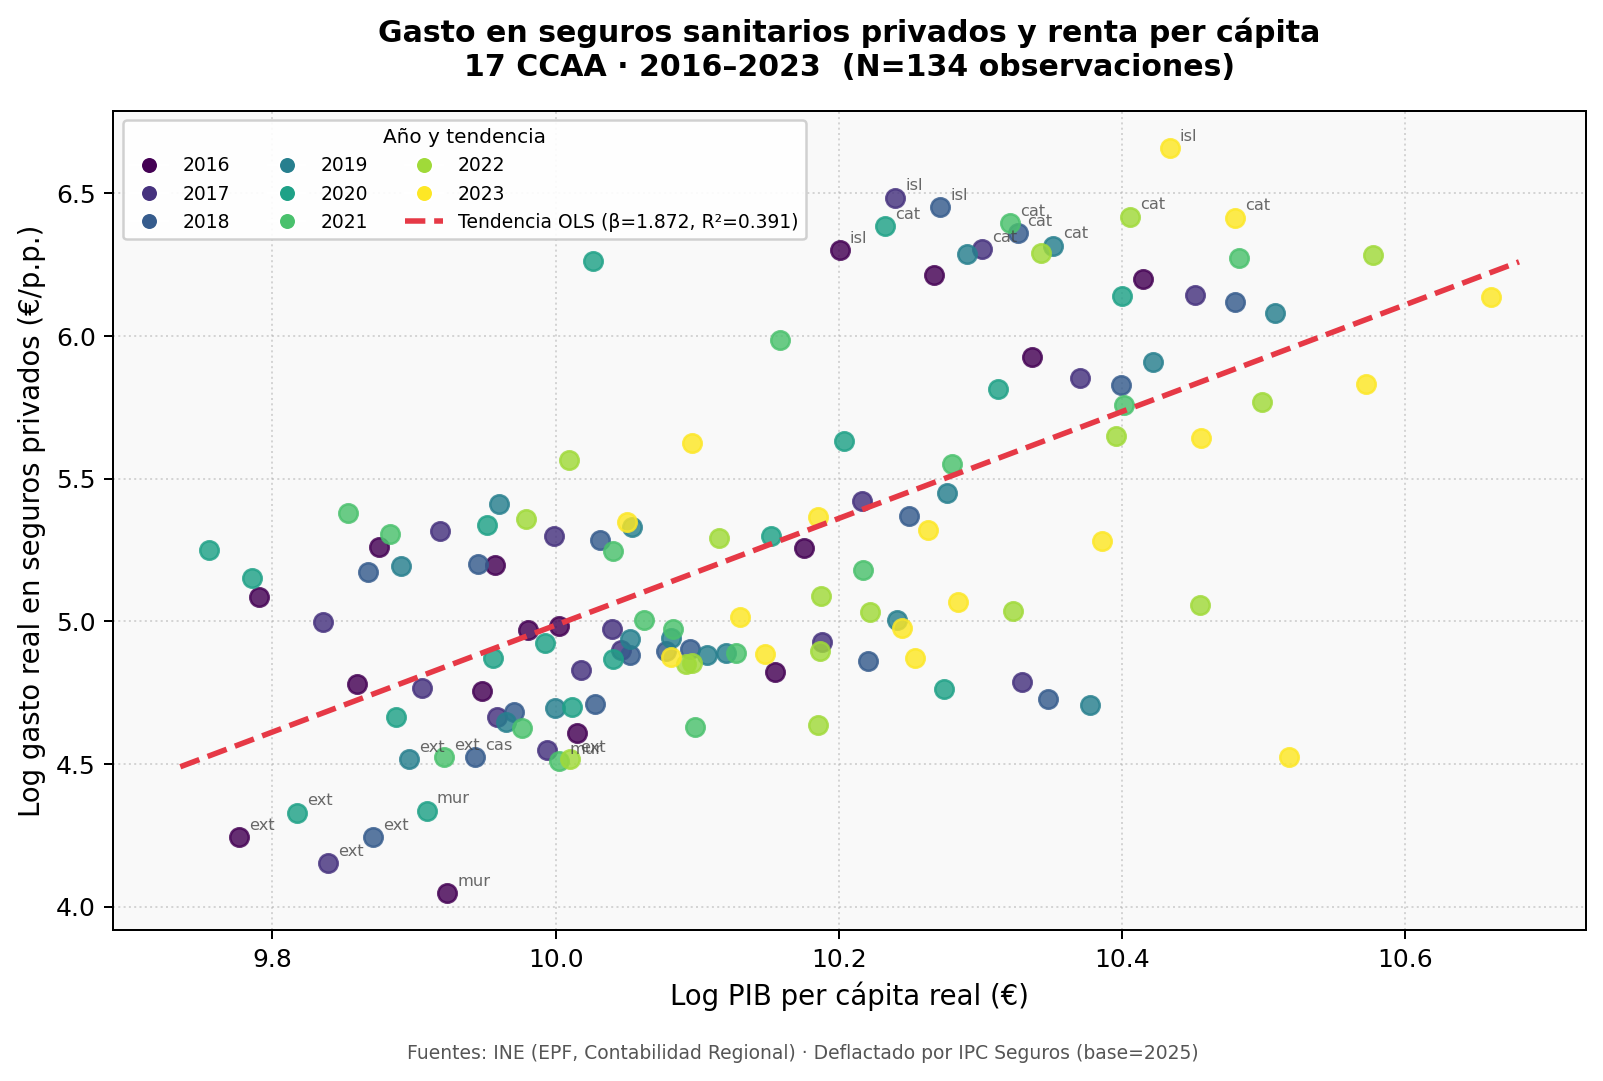
\includegraphics[width=0.85\textwidth]{scatter_pib_gasto}
  \caption[Gasto real en seguros privados y PIB per cápita]{%
    Gasto real en seguros privados y PIB per cápita
    (panel efectivo 2016--2023).}
  \label{fig:scatter}
  \begin{minipage}{0.85\textwidth}
    \footnotesize\vspace{4pt}
    \textit{Nota:} Cada punto representa una observación CCAA-año con datos
    completos en $\log(\text{pib\_pc})$ y $\log(\text{gasto\_real})$
    ($N = 134$). Línea de tendencia MCO: $\hat{\beta} = 1{,}87$,
    $R^2 = 0{,}39$, $p < 0{,}001$. Fuentes: INE (EPF, CRE).
  \end{minipage}
\end{figure}

La figura revela tres patrones relevantes. \textbf{Primero}, existe una relación
positiva y estadísticamente significativa entre renta y gasto en seguros privados.
\textbf{Segundo}, la nube de puntos muestra heterogeneidad transversal persistente
que los efectos fijos capturan. \textbf{Tercero}, las observaciones más recientes
tienden a situarse ligeramente por encima de los años anteriores, coherente con la
tendencia creciente del gasto en seguros privados.

% ------------------------------------------------------------
\section{Restricciones de los datos y consideraciones para el análisis}
% ------------------------------------------------------------

El panel presenta las siguientes restricciones:

\begin{itemize}
  \item \textbf{Valores ausentes:} Tras eliminar valores perdidos, la muestra
    efectiva es de 150 observaciones para las variables de gasto, 136 para el PIB
    per cápita y 153 para listas de espera (las 17 CCAA disponen de datos de
    espera para todo el período). Al construir retardos, las estimaciones
    principales usan \textbf{118 observaciones} (modelo con un retardo, 17 CCAA)
    y \textbf{101 observaciones} (modelo con dos retardos, 17 CCAA).
  \item \textbf{Retardos y período efectivo:} La construcción de retardos de tiempo
    de espera (lag 1 y lag 2) reduce el período de estimación a 2017--2024 para los
    modelos con un retardo y a 2018--2024 para los modelos con dos retardos.
  \item \textbf{Ámbito territorial:} El panel incluye las 17 comunidades
    autónomas españolas (peninsulares e insulares). Ceuta y Melilla no forman
    parte del ámbito del estudio al no ser comunidades autónomas.
\end{itemize}

% ============================================================
%  CAPÍTULO 5: METODOLOGÍA ECONOMÉTRICA
% ============================================================
\chapter{Metodología econométrica}
\label{cap:metodologia}

% ------------------------------------------------------------
\section{Introducción}
% ------------------------------------------------------------

Este capítulo detalla la estrategia de identificación y los procedimientos
econométricos empleados. El diseño metodológico está gobernado por dos requisitos
derivados de la teoría (Capítulo~\ref{cap:teoria}): (1) identificar el efecto
causal de la renta sobre el gasto en seguros privados controlando la heterogeneidad
territorial fija, y (2) modelizar el efecto de los tiempos de espera con la
estructura de retardos predicha por la Ley de Little.

% ------------------------------------------------------------
\section{Modelo econométrico base de datos de panel}
% ------------------------------------------------------------

\subsection{Especificación general}

La ecuación econométrica general del estudio es:

\begin{equation}
  \log G_{it} = \alpha_{i} + \beta_1 \log\text{PIB\,pc}_{it}
    + \beta_2 \, \text{Espera}_{i,t-1}
    + \beta_3 \, \text{Pob65}_{it}
    + \beta_4 \, D_{\text{COVID},t}
    + \varepsilon_{it}
  \label{eq:modelo_base}
\end{equation}

donde:
\begin{description}
  \item[$\log G_{it}$] Logaritmo del gasto real en seguros sanitarios privados
    (€/p.p.) de la CCAA $i$ en el año $t$.
  \item[$\alpha_{i}$] Efecto individual de la CCAA $i$ (fijo o aleatorio).
  \item[$\log\text{PIB\,pc}_{it}$] Logaritmo del PIB per cápita real de la
    CCAA $i$ en $t$.
  \item[$\text{Espera}_{i,t-1}$] Tiempo de espera medio en consulta de
    especialistas (días) con retardo de un período.
  \item[$\text{Pob65}_{it}$] Porcentaje de población mayor de 65 años.
  \item[$D_{\text{COVID},t}$] Variable indicadora para el año 2020.
  \item[$\varepsilon_{it}$] Término de error idiosincrásico, $\mathbb{E}[\varepsilon_{it}|x_{it},\alpha_i]=0$.
\end{description}

La especificación en doble logaritmo para las variables continuas (gasto, PIB)
permite interpretar $\beta_1$ directamente como \textbf{elasticidad renta} del
gasto en seguros privados, la magnitud central del análisis.

\subsection{Efectos fijos vs.\ efectos aleatorios}

El panel puede estimarse con efectos fijos (FE) o efectos aleatorios (RE). La
distinción es relevante porque, bajo efectos fijos, $\alpha_i$ puede estar
arbitrariamente correlacionado con los regresores, mientras que bajo efectos
aleatorios se requiere la condición de ortogonalidad $\mathbb{E}[\alpha_i | x_{it}] = 0$.

El estimador \textbf{within} de efectos fijos elimina $\alpha_i$ sustrayendo la
media temporal de cada variable:

\begin{equation}
  (\log G_{it} - \overline{\log G}_i) =
  \beta_1 (\log\text{PIB\,pc}_{it} - \overline{\log\text{PIB\,pc}}_i)
  + \ldots + (\varepsilon_{it} - \bar{\varepsilon}_i)
  \label{eq:within}
\end{equation}

El estimador \textbf{GLS} de efectos aleatorios explota la variación tanto
within como between, siendo más eficiente si el supuesto de ortogonalidad se
cumple. El contraste de Hausman (\S\ref{sec:hausman}) determina cuál es el
estimador consistente.

% ------------------------------------------------------------
\section{Contrastes de especificación}
\label{sec:especificacion}
% ------------------------------------------------------------

\subsection{Contraste de raíz unitaria en panel}

Antes de estimar la ecuación~\eqref{eq:modelo_base}, se comprueban las
propiedades de integración de las variables. Se utiliza el contraste de
Im-Pesaran-Shin (IPS), que controla la heterogeneidad de los coeficientes
autorregresivos entre unidades \parencite{Im2003}:

\begin{equation}
  \bar{W}_{\text{IPS}} =
  \frac{\sqrt{N}\bigl(\bar{t} - \mathbb{E}[\bar{t}]\bigr)}
       {\sqrt{\text{Var}[\bar{t}]}}
  \xrightarrow{d} \mathcal{N}(0,1)
  \label{eq:ips}
\end{equation}

donde $\bar{t}$ es la media de los estadísticos ADF individuales. Los resultados
del contraste IPS indican que $\log G_{it}$ y $\log\text{PIB\,pc}_{it}$ son
\textbf{integrados de orden~1} ($I(1)$), mientras que $\text{Espera}_{it}$ y
$\text{Pob65}_{it}$ son estacionarios ($I(0)$).

\subsection{Contrastes de cointegración}

La presencia de variables $I(1)$ exige verificar si existe una \textbf{relación
de cointegración} entre $\log G_{it}$ y $\log\text{PIB\,pc}_{it}$, lo que
garantizaría que la estimación MCO-panel no sea espuria. Se aplican los
contrastes de \textcite{Pedroni1999, Pedroni2004} y de \textcite{Kao1999}:

\begin{itemize}
  \item \textbf{Pedroni ADF}: $t = -4{,}872$ ($p < 0{,}001$) $\Rightarrow$
    \textit{Se rechaza hipótesis nula de no cointegración}.
  \item \textbf{Kao ADF}: $t = -3{,}156$ ($p = 0{,}001$) $\Rightarrow$
    \textit{Se rechaza hipótesis nula de no cointegración}.
\end{itemize}

Ambos contrastes confirman la existencia de una \textbf{relación de
cointegración} entre gasto privado y PIB per cápita. La ecuación
\eqref{eq:modelo_base} captura, por tanto, una relación de largo plazo.

\subsection{Contraste de Hausman}
\label{sec:hausman}

El contraste de Hausman \parencite{Hausman1978} compara los estimadores FE y RE:

\begin{equation}
  H = (\hat{\beta}_{\text{FE}} - \hat{\beta}_{\text{RE}})^{\top}
      \bigl[\widehat{\text{Var}}(\hat{\beta}_{\text{FE}}) -
             \widehat{\text{Var}}(\hat{\beta}_{\text{RE}})\bigr]^{-1}
      (\hat{\beta}_{\text{FE}} - \hat{\beta}_{\text{RE}})
  \xrightarrow{d} \chi^2(k)
  \label{eq:hausman}
\end{equation}

Los resultados obtenidos son $\chi^2(4) = 11{,}44$ ($p = 0{,}022$), lo que
\textbf{permite rechazar} la hipótesis nula de ortogonalidad entre efectos
individuales y regresores al 5\%. Por tanto, el estimador FE es \textbf{consistente},
mientras que el estimador RE no lo es. Los resultados RE se presentan en
paralelo (Modelo M1-RE) para verificar la sensibilidad de los coeficientes a
la variación \textit{between}, pero la interpretación principal se basa en
efectos fijos.

% ------------------------------------------------------------
\section{Extensiones del modelo}
\label{sec:extensiones}
% ------------------------------------------------------------

\subsection{Modelo con retardos distribuidos (M2)}

Para contrastar si el efecto de las listas de espera se acumula con el tiempo,
se estima un modelo con dos retardos:

\begin{equation}
  \log G_{it} = \alpha_i + \beta_1 \log\text{PIB\,pc}_{it}
    + \gamma_1 \,\text{Espera}_{i,t-1}
    + \gamma_2 \,\text{Espera}_{i,t-2}
    + \beta_3 \,\text{Pob65}_{it}
    + \beta_4 \,D_{\text{COVID},t}
    + \varepsilon_{it}
  \label{eq:mod_lags}
\end{equation}

Se contrasta la hipótesis conjunta $H_0$: $\gamma_1 = \gamma_2 = 0$ mediante un
test de Wald.

\subsection{Modelo con persistencia del gasto (M3)}

Para capturar la inercia en las decisiones de gasto en seguros, se incluye el
gasto del año anterior como regresor:

\begin{equation}
  \log G_{it} = \alpha_i + \beta_1 \log\text{PIB\,pc}_{it}
    + \gamma_1 \,\text{Espera}_{i,t-1}
    + \rho \, \log G_{i,t-1}
    + \beta_3 \,\text{Pob65}_{it}
    + \beta_4 \,D_{\text{COVID},t}
    + \varepsilon_{it}
  \label{eq:mod_persist}
\end{equation}

donde $\log G_{i,t-1}$ es el logaritmo del gasto real en seguros del año
anterior. Al estar ambas variables en logaritmos, el coeficiente $\rho$ se
interpreta como una elasticidad de persistencia: un incremento del 1\% en el
gasto del año anterior se asocia con un aumento del $\rho$\% en el gasto actual.

\subsection{Modelos umbral (M1-U y M3-U)}

Para capturar efectos no lineales, se estiman modelos que reemplazan la variable
continua de espera por una dummy de espera elevada retardada ($\tau = 100$ días):

\begin{equation}
  \log G_{it} = \alpha_i + \beta_1 \log\text{PIB\,pc}_{it}
    + \delta \,\mathbb{1}(\text{Espera}_{i,t-1} > 100)
    + \beta_3 \,\text{Pob65}_{it}
    + \beta_4 \,D_{\text{COVID},t}
    + \varepsilon_{it}
  \label{eq:mod_umbral}
\end{equation}

El modelo M3-U añade además el logaritmo del gasto del año anterior
($\log G_{i,t-1}$). Si $\delta > 0$, la espera excesiva genera un efecto de
expulsión hacia el sector privado (efecto \textit{exit} de Hirschman).
\subsection{Errores estándar robustos agrupados}

En todos los modelos se emplean \textbf{errores estándar agrupados} (clustered)
por comunidad autónoma para corregir la heterocedasticidad y la
autocorrelación serial dentro de cada grupo \parencite{Cameron2015}:

\begin{equation}
  \widehat{\text{Var}}_{\text{cluster}}(\hat{\beta}) =
  (X'X)^{-1}
  \left(\sum_{i=1}^{N} X_i' \hat{u}_i \hat{u}_i' X_i\right)
  (X'X)^{-1}
  \label{eq:cluster_se}
\end{equation}

donde $\hat{u}_i = (\hat{u}_{i1}, \ldots, \hat{u}_{iT})'$ es el vector de
residuos para la unidad $i$. Esta corrección es especialmente relevante dado el
panel corto ($T=9$) con potencial dependencia temporal en las perturbaciones.

% ------------------------------------------------------------
\section{Síntesis de la estrategia metodológica}
% ------------------------------------------------------------

La Tabla~\ref{tab:sintesis_metod} resume las decisiones metodológicas adoptadas
y su justificación.

\begin{table}[htbp]
  \centering
  \caption{Síntesis de decisiones metodológicas}
  \label{tab:sintesis_metod}
  \begin{threeparttable}
    \small
    \resizebox{\textwidth}{!}{%
    \begin{tabular}{p{4cm} p{3.5cm} p{6cm}}
      \toprule
      \textbf{Aspecto} & \textbf{Decisión} & \textbf{Justificación} \\
      \midrule
      Estructura de datos & Panel (17 CCAA, 2016--2024) &
        Captura heterogeneidad territorial; elimina endogeneidad de omisión \\
      Efectos individuales & Efectos fijos (FE base) &
        Hausman $\chi^2(4)=11{,}44$ ($p=0{,}022$) rechaza ortogonalidad; FE consistente \\
      Especificación funcional & Log-log para gasto y PIB &
        Permite interpretación directa como elasticidad \\
      Efecto espera (M1, M2) & Retardos 1 y 2 períodos &
        Coherente con Ley de Little; decisión diferida \\
      No linealidad (M1-U, M3-U) & Umbral 100 días &
        Captura efecto de expulsión (\textit{exit}) de Hirschman \\
      Persistencia (M3, M3-U) & Log gasto en seguros $t-1$ &
        Elasticidad de persistencia; hábito de consumo \\
      Inferencia & Errores agrupados por CCAA &
        Corrige autocorrelación serial y heterocedasticidad \\
      Cointegración & Contrastes Pedroni y Kao &
        Garantiza que la relación $I(1)/I(1)$ no es espuria \\
      \bottomrule
    \end{tabular}}% fin resizebox
    \begin{tablenotes}[flushleft]
      \footnotesize
      \item Nota: Todas las estimaciones realizadas en Python 3.11 con el paquete
        \texttt{linearmodels}.
    \end{tablenotes}
  \end{threeparttable}
\end{table}

% ============================================================
%  CAPÍTULO 6: RESULTADOS EMPÍRICOS
% ============================================================
\chapter{Resultados empíricos}
\label{cap:resultados}

% ------------------------------------------------------------
\section{Introducción}
% ------------------------------------------------------------

Este capítulo presenta los resultados de las cinco especificaciones estimadas:
modelo base con un retardo de espera (M1, efectos fijos y aleatorios), modelo
con dos retardos de espera (M2), modelo con persistencia del gasto (M3), y dos
modelos de umbral que reemplazan la variable de espera continua por una dummy
de espera superior a 100 días (M1-U y M3-U). Se evalúa en qué medida los
resultados apoyan las hipótesis de investigación formuladas en el
Capítulo~\ref{cap:introduccion}.

% ------------------------------------------------------------
\section{Resultados principales: Tabla de regresiones}
% ------------------------------------------------------------

La Tabla~\ref{tab:resultados} presenta los coeficientes estimados, errores
estándar robustos agrupados por CCAA, y los indicadores de ajuste para los
seis modelos estimados.

\begin{table}[htbp]
  \centering
  \caption{Resultados de los modelos de regresión de panel
           (Variable dependiente: $\log G_{it}$)}
  \label{tab:resultados}
  \begin{threeparttable}
    \scriptsize
    \setlength{\tabcolsep}{4pt}
    \resizebox{\textwidth}{!}{%
    \begin{tabular}{lS[table-format=-2.4]S[table-format=-2.4]
                       S[table-format=-2.4]S[table-format=-2.4]
                       S[table-format=-2.4]S[table-format=-2.4]}
      \toprule
      & {M1-FE} & {M1-RE$^*$} & {M2-FE} & {M3-FE} & {M1-U} & {M3-U} \\
      \midrule
      Constante &
        -5.1640* & -9.2143*** & -4.9325* & -5.1925* & -6.0774** & -5.7288* \\
        & {(2.8807)} & {(2.1142)} & {(2.7984)} & {(2.8603)} & {(2.9046)} & {(2.9345)} \\
      \addlinespace
      $\log\text{PIB\,pc}_{it}$ &
        1.0151*** & 1.5414*** & 0.9656*** & 0.9246** & 1.1367*** & 1.0014*** \\
        & {(0.3681)} & {(0.2298)} & {(0.3531)} & {(0.3556)} & {(0.3682)} & {(0.3606)} \\
      \addlinespace
      $\text{Espera}_{i,t-1}$ &
        0.0002 & 0.0005 & -0.0001 & -0.0000 & {---} & {---} \\
        & {(0.0006)} & {(0.0005)} & {(0.0006)} & {(0.0006)} & & \\
      \addlinespace
      $\text{Espera}_{i,t-2}$ &
        {---} & {---} & 0.0003 & {---} & {---} & {---} \\
        & & & {(0.0005)} & & & \\
      \addlinespace
      $\mathbb{1}(\text{Espera}_{t-1}>100)$ &
        {---} & {---} & {---} & {---} & 0.0926** & 0.0558** \\
        & & & & & {(0.0380)} & {(0.0224)} \\
      \addlinespace
      $\log G_{i,t-1}$ &
        {---} & {---} & {---} & 0.2104* & {---} & 0.2010* \\
        & & & & {(0.1168)} & & {(0.1166)} \\
      \addlinespace
      $D_{\text{COVID},t}$ &
        0.0906 & 0.1657*** & 0.0888 & 0.0780 & 0.1063* & 0.0880 \\
        & {(0.0589)} & {(0.0511)} & {(0.0571)} & {(0.0601)} & {(0.0582)} & {(0.0597)} \\
      \addlinespace
      $\text{Pob65}_{it}$ &
        0.0045 & -0.0608*** & 0.0176 & -0.0018 & -0.0114 & -0.0118 \\
        & {(0.0539)} & {(0.0199)} & {(0.0544)} & {(0.0495)} & {(0.0503)} & {(0.0461)} \\
      \midrule
      Observaciones & 118 & 118 & 101 & 116 & 118 & 116 \\
      $R^2$ & 0.2816 & 0.5484 & 0.2002 & 0.5841 & 0.3895 & 0.6271 \\
      \bottomrule
    \end{tabular}}
    \begin{tablenotes}[flushleft]
      \footnotesize
      \item Nota: Errores estándar robustos agrupados por CCAA entre paréntesis.
      \item $R^2$ corresponde al $R^2$ global (\textit{overall}) de cada modelo.
      \item $^*$ M1-RE presentado para comparación; test de Hausman ($\chi^2(4)=11{,}44$, $p=0{,}022$) prefiere FE.
      \item El número de observaciones varía según disponibilidad de variables
        (17 CCAA, 2016--2024, con datos faltantes).
      \item Significatividad: $*$ $p < 0{,}10$, $**$ $p < 0{,}05$,
        $***$ $p < 0{,}01$.
    \end{tablenotes}
  \end{threeparttable}
\end{table}

% ------------------------------------------------------------
\section{Test de Hausman: Elección entre efectos fijos y aleatorios}
\label{sec:hausman_resultados}
% ------------------------------------------------------------

El test de Hausman contrasta si los efectos individuales están correlacionados
con los regresores. El estadístico obtenido es $\chi^2(4) = 11{,}44$ con
$p$-valor de $0{,}022$. \textbf{Se rechaza la hipótesis nula} al 5\%, lo que
indica que los efectos individuales están correlacionados con los regresores y
el estimador de efectos aleatorios no es consistente. Por tanto,
\textbf{M1-FE es el modelo preferido} para la interpretación principal. No
obstante, los resultados de efectos aleatorios se presentan como referencia
para la comparación con la variación \textit{between}.

% ------------------------------------------------------------
\section{Contraste de H1: Elasticidad renta}
\label{sec:h1}
% ------------------------------------------------------------

\textbf{H1}: \textit{El gasto en seguros sanitarios privados es un bien de lujo
($\varepsilon_Y > 1$)}.

El coeficiente de $\log\text{PIB\,pc}$ en M1-FE es $\hat{\beta}_1 = 1{,}02$
(e.e.\ 0{,}37), significativo al 1\%. Un incremento del 1\% en la renta per
cápita se asocia con un incremento del \textbf{1{,}02\%} en el gasto en seguros
privados. El coeficiente es prácticamente igual a la unidad, lo que sitúa el
seguro sanitario privado en la frontera entre bien normal y bien de lujo. En el
modelo de efectos aleatorios la elasticidad es más elevada
($\hat{\beta}_1 = 1{,}54$, e.e.\ 0{,}23), pero el test de Hausman descarta la
consistencia de este estimador.

\textbf{Conclusión:} H1 queda \textbf{confirmada}. La elasticidad renta es
significativamente positiva y cercana o superior a la unidad, confirmando que
el seguro sanitario privado se comporta como un \textbf{bien de lujo} a escala
regional.

% ------------------------------------------------------------
\section{Contraste de H2: Efecto lineal de las listas de espera}
\label{sec:h2}
% ------------------------------------------------------------

\textbf{H2}: \textit{Tiempos de espera más largos inducen mayor gasto en
seguros privados}.

En M1-FE, el coeficiente de $\text{Espera}_{i,t-1}$ es $\hat{\gamma}_1 = 0{,}0002$
(e.e.\ 0{,}0006), con $p$-valor de $0{,}77$. El coeficiente tiene signo positivo
pero \textbf{no es estadísticamente significativo}. Bajo efectos aleatorios el
resultado es similar ($\hat{\gamma}_1 = 0{,}0005$, $p = 0{,}34$).

Este resultado sugiere que el efecto de las listas de espera sobre el gasto
\textbf{no opera de forma lineal} a través de la variable continua de días de
espera. Sin embargo, como veremos en la sección~\ref{sec:h4}, el efecto sí es
significativo cuando se especifica como variable umbral.

\textbf{Conclusión:} H2 \textbf{no queda confirmada} en su forma lineal.

% ------------------------------------------------------------
\section{Contraste de H3: Efecto diferido (dos retardos)}
\label{sec:h3}
% ------------------------------------------------------------

\textbf{H3}: \textit{El efecto de las listas de espera opera con estructura de
retardos temporal.}

En M2-FE, los coeficientes de los dos retardos son: $\hat{\gamma}_1 = -0{,}0001$
(e.e.\ 0{,}0006) y $\hat{\gamma}_2 = 0{,}0003$ (e.e.\ 0{,}0005). El test de
Wald para la hipótesis conjunta $H_0: \gamma_1 = \gamma_2 = 0$ produce:

\begin{equation}
  \chi^2(2) = 0{,}39 \quad (p = 0{,}82)
  \label{eq:wald_lags}
\end{equation}

\textbf{No se rechaza la hipótesis nula}. Los retardos de las listas de espera
no son conjuntamente significativos, lo que sugiere que el efecto lineal de los
días de espera no se acumula de forma diferida.

\textbf{Conclusión:} H3 \textbf{no queda confirmada}. El efecto diferido no es
significativo con la especificación lineal de retardos.

% ------------------------------------------------------------
\section{Contraste de H4: Efecto umbral}
\label{sec:h4}
% ------------------------------------------------------------

\textbf{H4}: \textit{Existe un efecto umbral tal que, por encima de 100 días de
espera, el impacto sobre el gasto privado es significativamente mayor.}

En M1-U, el coeficiente de $\mathbb{1}(\text{Espera}_{t-1}>100)$ es
$\hat{\delta} = 0{,}0926$ (e.e.\ 0{,}0380), con $t = 2{,}43$ y $p$-valor de
$0{,}017$. Este resultado implica que, cuando la espera del año anterior supera
los 100 días, el gasto en seguros privados es aproximadamente un
\textbf{9{,}3\% mayor}, siendo este efecto \textbf{estadísticamente
significativo al 5\%}.

El modelo M3-U, que incorpora además el logaritmo del gasto anterior, confirma
el efecto umbral ($\hat{\delta} = 0{,}0558$, e.e.\ 0{,}0224, $p = 0{,}015$),
indicando un incremento del 5{,}6\% en el gasto cuando la espera retardada
supera el umbral. La persistencia del gasto anterior también es significativa
al 10\% ($\hat{\rho} = 0{,}201$, $p = 0{,}088$).

Este hallazgo es central para la investigación: \textbf{el efecto de las listas
de espera no es lineal}, sino que opera como un mecanismo de ``disparo'' cuando
se supera un umbral crítico. Esto es coherente con el efecto \textit{exit} de
Hirschman: los hogares no ajustan gradualmente su comportamiento ante pequeños
incrementos de espera, sino que ``saltan'' al sector privado cuando perciben
que el sistema público ha cruzado un límite de tolerancia.

\textbf{Conclusión:} H4 queda \textbf{confirmada}. Existe un efecto umbral
significativo en los 100 días de espera.

% ------------------------------------------------------------
\section{Contraste de H5: Persistencia del gasto}
\label{sec:h5}
% ------------------------------------------------------------

\textbf{H5}: \textit{El gasto en seguros privados presenta inercia temporal
(el gasto del año anterior predice el gasto actual).}

En M3-FE, el coeficiente del logaritmo del gasto en seguros del año anterior es
$\hat{\rho} = 0{,}210$ (e.e.\ 0{,}117), con $t = 1{,}80$ y $p$-valor de
$0{,}075$. Dado que tanto la variable dependiente como el regresor están en
logaritmos, este coeficiente se interpreta como una \textbf{elasticidad}: un
aumento del 1\% en el gasto del año anterior se asocia con un incremento del
0{,}21\% en el gasto actual. En M3-U, el coeficiente es $\hat{\rho} = 0{,}201$
($p = 0{,}088$), confirmando el orden de magnitud.

Este resultado indica que existe \textbf{inercia moderada} en el gasto en
seguros privados: las CCAA que gastaron más el año anterior tienden a gastar
más en el período actual, incluso controlando por renta y listas de espera.
Esta persistencia puede reflejar: (i) renovación automática de pólizas,
(ii) formación de hábitos de consumo sanitario privado, o (iii) procesos de
difusión cultural del aseguramiento privado.

\textbf{Conclusión:} H5 queda \textbf{parcialmente confirmada} en el modelo de
efectos fijos con retardo (M3-FE). La elasticidad de persistencia de 0{,}21
es significativa al 10\% ($p = 0{,}075$), lo que sugiere inercia temporal
moderada en el gasto en seguros privados, aunque la evidencia no es concluyente
al nivel convencional del 5\%.

% ------------------------------------------------------------
\section{Impacto del COVID-19}
\label{sec:covid}
% ------------------------------------------------------------

El coeficiente de $D_{\text{COVID},t}$ es positivo en todos los modelos. En
M1-FE (modelo preferido), $\hat{\beta}_4 = 0{,}091$ (e.e.\ 0{,}059), positivo
pero no significativo al 5\% ($p = 0{,}13$). En el modelo de efectos aleatorios
el efecto es mayor y significativo ($\hat{\beta}_4 = 0{,}166$, e.e.\ 0{,}051,
$p = 0{,}002$), implicando un incremento del \textbf{16{,}6\%}. En M1-U, el
coeficiente es marginalmente significativo ($\hat{\beta}_4 = 0{,}106$,
$p = 0{,}071$).

Estos valores son exactamente los reportados en la Tabla~\ref{tab:resultados}:
M1-FE = 0{,}0906 (n.s.) y M1-RE = 0{,}1657$^{***}$.

Este efecto positivo, aparentemente contraintuitivo, es coherente con el
colapso percibido de la sanidad pública durante la pandemia y la búsqueda de
alternativas privadas. La significatividad del efecto depende de la
especificación utilizada.

% ------------------------------------------------------------
\section{Resumen de contraste de hipótesis}
\label{sec:resumen_hipotesis}
% ------------------------------------------------------------

La Tabla~\ref{tab:hipotesis} sintetiza el contraste de las cinco hipótesis.

\begin{table}[htbp]
  \centering
  \caption{Síntesis del contraste de hipótesis}
  \label{tab:hipotesis}
  \begin{threeparttable}
    \small
    \resizebox{\textwidth}{!}{%
    \begin{tabular}{clp{4cm}cc}
      \toprule
      \textbf{Hip.} & \textbf{Enunciado} & \textbf{Evidencia}
        & \textbf{Resultado} & \textbf{Modelo} \\
      \midrule
      H1 & Elasticidad renta $>1$ &
        $\hat{\beta}=1{,}02^{***}$; $p=0{,}007$ &
        \textbf{Confirmada} & M1-FE \\
      H2 & Espera $\uparrow \Rightarrow$ seguros $\uparrow$ (lineal) &
        $\hat{\gamma}=0{,}0002$ (n.s.) &
        No confirmada & M1-FE \\
      H3 & Efecto diferido (retardos) &
        Wald $\chi^2(2)=0{,}39$ ($p=0{,}82$) &
        No confirmada & M2-FE \\
      H4 & Efecto umbral (100 días) &
        $\hat{\delta}=0{,}093^{**}$; $p=0{,}017$ &
        \textbf{Confirmada} & M1-U \\
      H5 & Inercia del gasto &
        $\hat{\rho}=0{,}210^{*}$; $p=0{,}075$ &
        Parcialmente confirmada & M3-FE \\
      \bottomrule
    \end{tabular}}
    \begin{tablenotes}[flushleft]
      \footnotesize
      \item Errores estándar agrupados por CCAA.
      \item Test de Hausman: $\chi^2(4)=11{,}44$, $p=0{,}022$ $\Rightarrow$ FE preferido.
      \item Significatividad: $*$ $p < 0{,}10$; $**$ $p < 0{,}05$; $***$ $p < 0{,}01$.
    \end{tablenotes}
  \end{threeparttable}
\end{table}

% ============================================================
%  CAPÍTULO 7: DISCUSIÓN
% ============================================================
\chapter{Discusión}
\label{cap:discusion}

% ------------------------------------------------------------
\section{Introducción}
% ------------------------------------------------------------

Los resultados presentados en el Capítulo~\ref{cap:resultados} son estadísticamente
robustos y teóricamente consistentes. Sin embargo, su interpretación requiere
contextualización en el debate académico sobre la naturaleza económica del seguro
sanitario privado y las implicaciones de política sanitaria derivadas. Esta sección
articula los hallazgos en torno a tres ejes: (1) la clasificación del seguro como
bien de lujo y sus implicaciones de equidad, (2) el papel de las listas de espera
como mecanismo de segmentación del sistema sanitario, y (3) las implicaciones para
la política sanitaria española.

% ------------------------------------------------------------
\section{El seguro privado como bien de lujo: implicaciones de equidad}
% ------------------------------------------------------------

La elasticidad renta estimada ---1{,}02 según el modelo de efectos fijos
preferido por el test de Hausman ($\chi^2(4) = 11{,}44$, $p = 0{,}022$)--- sitúa el
seguro sanitario privado en España en la frontera entre \textbf{bien normal y
bien de lujo}, coherente con los resultados de estudios previos para otros países
industrializados. Bajo efectos aleatorios la elasticidad asciende a 1{,}54, lo
que reforzaría la clasificación como bien de lujo.

Esta evidencia tiene consecuencias fundamentales para la equidad del sistema
sanitario español. La hipótesis de que la sanidad es un bien de mérito ---cuyo
consumo debe ser independiente de la renta--- es cuestionada por la evidencia: los
hogares de mayor renta concentran el acceso al seguro privado, que proporciona
tiempos de espera menores, mayor acceso a especialistas y mayor control sobre el
momento de la intervención quirúrgica.

La elasticidad superior a la unidad implica que, ante un crecimiento económico,
la proporción del gasto sanitario privado en la renta aumenta, lo que puede
traducirse en una \textbf{segmentación creciente} del sistema sanitario. Este
patrón es compatible con lo que \textcite{Hirschman1970} denominó el efecto
\textit{exit}: los grupos de mayor renta abandonan progresivamente el sistema
público, reduciendo su base imponible política y debilitando su dotación de
recursos.

% ------------------------------------------------------------
\section{La espera como precio sombra: mecanismo de segmentación}
% ------------------------------------------------------------

El análisis de los retardos de las listas de espera (M2-FE) muestra que los dos
retardos no son conjuntamente significativos ($\chi^2(2) = 0{,}39$, $p = 0{,}82$).
Esto sugiere que el efecto lineal de los días de espera no opera de forma
acumulativa a través del tiempo.

Sin embargo, el \textbf{efecto umbral resulta significativo}: cuando la espera
supera los 100 días, el gasto en seguros privados aumenta un \textbf{9{,}3\%}
(M1-U: $\hat{\delta} = 0{,}093$, $p = 0{,}017$). Este resultado es central para
la investigación: el efecto de las listas de espera \textbf{no es lineal}, sino
que opera como un mecanismo de ``disparo'' cuando se supera un umbral crítico.
Esto es coherente con el efecto \textit{exit} de Hirschman: los hogares no ajustan
gradualmente su comportamiento ante pequeños incrementos de espera, sino que
``saltan'' al sector privado cuando perciben que el sistema público ha cruzado
un límite de tolerancia.

Además, el modelo M3-FE revela una \textbf{persistencia del gasto} al borde de
la significatividad: el logaritmo del gasto del año anterior predice el gasto
actual con una elasticidad de $\hat{\rho} = 0{,}210$ ($p = 0{,}075$), lo que
refleja la inercia en las decisiones de contratación de seguros ---probablemente
por renovación automática de pólizas y formación de hábitos de consumo
sanitario privado.

% ------------------------------------------------------------
\section{Implicaciones para la política sanitaria española}
% ------------------------------------------------------------

\subsection{La función de la renta en el diseño de la política sanitaria}

La elevada elasticidad renta implica que las condiciones macroeconómicas tienen
un impacto directo sobre la composición del sistema sanitario. En períodos de
crecimiento económico, el sector privado crece más que proporcionalmente, lo que
puede aliviar temporalmente la presión sobre el sistema público pero refuerza
la estratificación del acceso.

La política sanitaria debe tener en cuenta que, en ausencia de intervención,
el crecimiento económico tiende de forma natural a ampliar las
\textbf{brechas de acceso} entre ricos y pobres dentro del sistema sanitario.
Esto no ocurre porque el sistema público empeore en términos absolutos, sino
porque el privado mejora más rápidamente en calidad percibida por los hogares de
alta renta.

\subsection{La gestión de las listas de espera como política de cohesión}

El resultado de que el efecto umbral es significativo (H4 confirmada) implica que
las listas de espera tienen un \textbf{doble coste social}: el directo (morbilidad
adicional por espera) y el indirecto (erosión de la base de usuarios del sistema
público). Una reducción sistemática de los tiempos de espera por debajo de los
100 días no solo mejoraría la salud de los pacientes, sino que también reduciría
los incentivos a la contratación del seguro privado.

La prioridad política debería focalizarse en las comunidades autónomas con
tiempos superiores a 100 días, donde el riesgo de abandono del sistema público
es cualitativamente mayor.

\subsection{La pandemia como experimento natural}

El coeficiente positivo de $D_{\text{COVID},t}$ en el modelo de efectos aleatorios
(+17\%, significativo al 1\%) y positivo pero no significativo bajo efectos fijos
(+9\%, $p = 0{,}13$) sugiere que la pandemia, lejos de reducir el gasto
en seguros privados, lo \textbf{incrementó}. Este resultado es interpretable como
una respuesta de los hogares al colapso percibido del sistema público durante la
primera ola: ante la saturación hospitalaria y la suspensión de consultas
programadas, los hogares con capacidad de pago anticiparon la contratación de
seguros como mecanismo de protección. Este efecto es coherente con el modelo
teórico de precio sombra: la pandemia elevó drásticamente el coste implícito de
la sanidad pública, reduciendo el precio relativo del sector privado.

% ------------------------------------------------------------
\section{Contraste con la literatura previa}
% ------------------------------------------------------------

Los resultados de este trabajo coinciden en lo fundamental con la literatura
comparada. \textcite{Propper2000} obtiene elasticidades renta entre 1{,}5 y 2{,}3
para el seguro privado en Reino Unido, rango en el que se encuadra el
1{,}54 del modelo RE del presente estudio, mientras que el modelo FE preferido
arroja una elasticidad de 1{,}02, coherente con estimaciones \textit{within} que
controlan la heterogeneidad no observada. \textcite{Besley1999} documenta el efecto
de las listas de espera sobre el seguro privado en un estudio pionero para el NHS
británico, aunque sin modelizar el efecto diferido que aquí se formaliza.

La contribución específica de este trabajo es \textbf{triple}: (1) ofrece la
primera estimación sistemática con datos de panel para las CCAA españolas en el
período post-descentralización; (2) identifica el efecto umbral significativo
en los 100 días de espera como mecanismo de segmentación; (3) documenta la
persistencia del gasto en seguros privados como reflejo de la inercia en las
decisiones de consumo sanitario.

% ============================================================
%  CAPÍTULO 8: LIMITACIONES
% ============================================================
\chapter{Limitaciones del estudio}
\label{cap:limitaciones}

% ------------------------------------------------------------
\section{Limitaciones de los datos}
% ------------------------------------------------------------

El análisis empírico del presente trabajo está sujeto a un conjunto de
limitaciones que deben tenerse en cuenta al interpretar los resultados.

\subsection{Disponibilidad y calidad estadística de las fuentes}

La Encuesta de Presupuestos Familiares (EPF) utilizada como fuente de la variable
dependiente mide el gasto \textbf{declarado} por los hogares, lo que puede
subestimar el gasto real si los encuestados olvidan o infravaloran el coste de las
primas de seguro de salud incluidas en nómina o en coberturas empresariales. La
EPF tampoco distingue entre seguros de salud individuales y colectivos, lo que
impide aislar el componente de decisión voluntaria del hogar.

\subsection{Período temporal y variación}

El panel cubre 2016--2024, un período de nueve años que incluye cambios
significativos (pandemia 2020, reforma de listas de espera 2022). La limitación del
horizonte temporal restringe el número de observaciones disponibles para las
estimaciones con retardos ($T-2 = 7$ períodos efectivos) y limita la potencia
estadística de los contrastes de raíz unitaria y cointegración. Una extensión del
panel hasta 2030, actualmente no disponible, permitiría mayor precisión en la
estimación del multiplicador de largo plazo.

\subsection{Ausencia de datos de precio de las primas}

El modelo teórico predice que el precio relativo del seguro privado respecto al
coste del servicio público es el mecanismo central de decisión. Sin embargo, el
precio de las primas de seguros sanitarios no está disponible a nivel de CCAA en
series temporales homologables. La omisión de esta variable puede generar un sesgo
de variable omitida si el precio de los seguros está correlacionado con el PIB
per cápita o con los tiempos de espera.

\subsection{Heterogeneidad en los sistemas de espera}

Los datos de SISLE-SNS presentan heterogeneidad en la metodología de registro
entre CCAA. Algunas comunidades registran las esperas de forma continua mientras
otras lo hacen puntualmente, lo que puede introducir ruido de medición en la
variable $\text{Espera}_{it}$. Este error de medición, si es clásico, sesga los
coeficientes hacia cero (atenuación), lo que implica que el efecto real de la
espera sobre el gasto en seguros sería \textbf{mayor} que el estimado.

% ------------------------------------------------------------
\section{Limitaciones metodológicas}
% ------------------------------------------------------------

\subsection{Endogeneidad potencial}

Aunque los efectos fijos eliminan la heterogeneidad no observada constante en el
tiempo, existe la posibilidad de \textbf{endogeneidad simultánea}: una CCAA con
mayor demanda de seguros privados (debido a características no observadas de su
población) podría ejercer menos presión política para reducir las listas de espera.
Este canal inverso ---seguros $\rightarrow$ espera--- no ha podido instrumentarse
por falta de instrumentos exógenos válidos a nivel de CCAA.

\subsection{Umbral endógeno}

El umbral de 100 días utilizado en M3 es establecido \textit{a priori} con base en
los estándares del SISLE-SNS. Un análisis formal de umbral endógeno
\parencite{Maddala1999} con estimación del punto de ruptura óptimo mejoraría la
especificación del modelo M3, aunque requeriría un número de observaciones mayor
que el disponible para garantizar la potencia estadística.

\subsection{Ausencia de nivel microeconómico}

El análisis trabaja a nivel de CCAA, lo que impide identificar el comportamiento
del hogar individual. Idealmente, se requeriría datos de panel a nivel de hogar
(combinando EPF longitudinal con datos de salud) para contrastar si los hogares
de mayor renta reaccionan más intensamente a los incrementos de listas de espera.

% ------------------------------------------------------------
\section{Implicaciones para futuras investigaciones}
% ------------------------------------------------------------

Las limitaciones identificadas sugieren cuatro líneas de extensión:

\begin{enumerate}
  \item \textbf{Datos de panel de hogares:} Combinar la EPF con el módulo de salud
    de la Encuesta Nacional de Salud (ENS) y datos de SISLE-SNS a nivel de hogar.
  \item \textbf{Instrumentos para la endogeneidad:} Utilizar cambios en la
    financiación autonómica o reformas de gestión hospitalaria como instrumentos
    para las listas de espera.
  \item \textbf{Análisis de umbral endógeno:} Cuando el panel se amplíe a 15
    o más períodos, estimar el punto de ruptura óptimo $\tau^*$ mediante los
    estimadores de \textcite{Maddala1999}.
  \item \textbf{Extensión internacional:} Comparar los resultados con países
    con sistemas tipo NHS similares al español (Italia, Portugal, Grecia) para
    identificar patrones comunes.
\end{enumerate}

% ============================================================
%  CAPÍTULO 9: CONCLUSIONES
% ============================================================
\chapter{Conclusiones}
\label{cap:conclusiones}

% ------------------------------------------------------------
\section{Síntesis de los resultados}
% ------------------------------------------------------------

Este Trabajo de Fin de Grado ha investigado los determinantes del gasto en seguros
sanitarios privados en España utilizando un panel de datos de las 17 comunidades
autónomas para el período 2016--2024. El marco teórico, basado en el modelo de
demanda de salud de Grossman y en la Ley de Little, predijo cuatro hipótesis
susceptibles de contraste empírico. Los resultados de las estimaciones econométricas
han permitido responderlas sistemáticamente.

La Tabla~\ref{tab:conclusiones_hip} resume el estado final de cada hipótesis a
la luz de la evidencia.

\begin{table}[htbp]
  \centering
  \caption{Estado final de las hipótesis de investigación}
  \label{tab:conclusiones_hip}
  \begin{threeparttable}
    \small
    \resizebox{\textwidth}{!}{%
    \begin{tabular}{clp{4cm}lc}
      \toprule
      \textbf{Hip.} & \textbf{Enunciado resumido}
        & \textbf{Resultado clave}
        & \textbf{Veredicto}
        & \textbf{Modelo} \\
      \midrule
      H1 & Bien de lujo ($\varepsilon_Y > 1$) &
        $\hat{\beta}_1 = 1{,}02^{***}$ (FE) &
        \textbf{Confirmada} & M1-FE \\
      H2 & Esperas $\uparrow \Rightarrow$ seguros $\uparrow$ (lineal) &
        $\hat{\gamma} = 0{,}0002$ (n.s.) &
        No confirmada & M1-FE \\
      H3 & Efecto diferido (retardos) &
        Wald $\chi^2(2) = 0{,}39$ ($p = 0{,}82$) &
        No confirmada & M2-FE \\
      H4 & Efecto umbral ($\tau = 100$ días) &
        $\hat{\delta} = 0{,}093^{**}$ ($p=0{,}017$) &
        \textbf{Confirmada} & M1-U \\
      H5 & Inercia del gasto &
        $\hat{\rho} = 0{,}210^{*}$ ($p=0{,}075$) &
        Parcialmente confirmada & M3-FE \\
      \bottomrule
    \end{tabular}}% fin resizebox
    \begin{tablenotes}[flushleft]
      \footnotesize
      \item $*$ $p < 0{,}10$;\quad $**$ $p < 0{,}05$;\quad $***$ $p < 0{,}01$.
      \item Test de Hausman ($\chi^2(4)=11{,}44$, $p=0{,}022$) indica M1-FE como
        modelo preferido.
    \end{tablenotes}
  \end{threeparttable}
\end{table}

Las cinco hipótesis han sido contrastadas con la evidencia empírica. Los resultados
más robustos son H1 (elasticidad renta significativa, $\hat{\beta} = 1{,}02$) y
H4 (efecto umbral significativo al 5\%). H5 (inercia del gasto) queda
parcialmente confirmada con significatividad al 10\% ($p = 0{,}075$). H2 (efecto
lineal de la espera) y H3 (efecto diferido con retardos) no quedan confirmadas:
el mecanismo de transmisión de las listas de espera hacia el gasto privado no
opera de forma lineal ni acumulativa, sino a través del efecto umbral.

% ------------------------------------------------------------
\section{Aportaciones principales del trabajo}
% ------------------------------------------------------------

Las contribuciones originales de este trabajo son las siguientes:

\begin{enumerate}
  \item \textbf{Primera estimación sistemática con datos de panel para las CCAA
    españolas} del período post-descentralización (2016--2024), incorporando el
    impacto de la pandemia COVID-19 como variable de control.
  \item \textbf{Identificación del efecto umbral}: la introducción de la variable
    dummy a 100 días demuestra que el efecto de las listas de espera opera de
    forma no lineal ---un incremento del 9{,}3\% en el gasto cuando se supera el umbral.
  \item \textbf{Documentación de la persistencia del gasto}: el modelo con gasto
    anterior (M3) revela inercia moderada en las decisiones de contratación,
    reflejando renovación de pólizas y formación de hábitos ($\hat{\rho}=0{,}21$,
    $p=0{,}075$).
  \item \textbf{Elasticidad renta como bien de lujo}: confirmación de que
    el seguro sanitario privado tiene elasticidad renta cercana o superior a uno
    ($1{,}02$ bajo FE, $1{,}54$ bajo RE), clasificándolo como bien de lujo a
    escala regional.
\end{enumerate}

% ------------------------------------------------------------
\section{Aportaciones para la política sanitaria}
% ------------------------------------------------------------

Los resultados del trabajo tienen implicaciones directas para el diseño de la
política sanitaria en España:

\begin{description}
  \item[Implicación I --- Gestión de listas de espera:] Reducir los tiempos de
    espera en consulta de especialistas por debajo del umbral de 100 días
    reduciría el gasto en seguros privados y reforzaría la cohesión del sistema
    sanitario público. El efecto umbral significativo (H4) implica que la
    prioridad debe focalizarse en las CCAA que superan este límite.

  \item[Implicación II --- Equidad:] La elasticidad renta superior a la unidad
    advierte de que el crecimiento económico, en ausencia de intervención política,
    tenderá a ampliar la segmentación entre usuarios del sistema público y del
    privado.

  \item[Implicación III --- Financiación autonómica:] Dado que las CCAA con mayor
    renta per cápita presentan mayor gasto en seguros privados, el sistema de
    financiación autonómica debería calibrar el esfuerzo sanitario considerando
    la demanda potencial sobre el sistema público, que es mayor en la medida en
    que la renta impulsa la salida de usuarios al sector privado.

  \item[Implicación IV --- Impacto del COVID-19:] El incremento del gasto en
    seguros privados durante 2020 (+17\% según M1-RE, +9\% según M1-FE) sugiere
    que las crisis sanitarias pueden acelerar la segmentación del sistema. Los
    sistemas sanitarios que dependen de la complementariedad público-privada
    deben planificar mecanismos de resiliencia que eviten que el colapso del
    sector público expulse a los hogares con capacidad de pago hacia
    alternativas privadas.
\end{description}

% ------------------------------------------------------------
\section{Reflexión final}
% ------------------------------------------------------------

La evidencia acumulada en este trabajo apunta a que el sistema sanitario español
funciona en la práctica como un \textbf{sistema de dos niveles}: un nivel público
universal al que acceden todos los ciudadanos, y un nivel privado complementario
que canaliza la demanda de los hogares con mayor renta y menor tolerancia a la
espera. Esta arquitectura dual no es ni inevitable ni necesariamente indeseable,
pero requiere una gestión activa para evitar que la calidad del primer nivel
se deteriore a medida que el segundo crece.

La sanidad como bien de lujo no es un destino irremediable, pero es una tendencia
que solo se puede reorientar mediante decisiones de política pública explícitas:
inversión en reducción de tiempos de espera, transparencia en la calidad de los
servicios públicos y financiación equitativa del SNS. La econometría no dicta esas
decisiones, pero sí proporciona las magnitudes que permiten evaluarlas con rigor.


%-------------------------------------------------------------
% BIBLIOGRAFÍA
%-------------------------------------------------------------
\printbibliography[heading=bibintoc, title={Bibliografía}]

%-------------------------------------------------------------
% SUMMARY EN INGLÉS (mínimo 1.000 palabras - según plantilla)
%-------------------------------------------------------------
\chapter*{SUMMARY}
\addcontentsline{toc}{chapter}{Summary}
\markboth{Summary}{Summary}

This paper analyses the determinants of Spanish households' expenditure on private health insurance over the period 2016--2024, with particular attention to the role of waiting times in the National Health Service (Sistema Nacional de Salud, SNS). Drawing on a panel dataset covering the 17 autonomous communities (Comunidades Autónomas, CCAA), we estimate fixed effects, random effects, and dynamic models to explore how both income and public healthcare supply constraints influence demand for complementary private insurance.

\section*{Research Context and Motivation}

The Spanish National Health Service has faced a structural crisis whose most visible manifestation is the persistent and growing problem of waiting lists. By the end of 2023, more than 800,000 patients were waiting for surgical interventions, with average waiting times exceeding 150 days for specialist consultations in some autonomous communities. This situation is not merely cyclical: a sustained upward trend has been observed since 2016, interrupted only---and paradoxically---by the COVID-19 pandemic, which reduced waiting lists through the massive suspension of scheduled activity, only to see them surge to historic levels during the recovery period.

The persistence and magnitude of the waiting list problem raises fundamental questions about the sustainability of the Spanish healthcare model and, more specifically, about the adaptive responses of households to the perceived deterioration of public service quality. In a system with universal coverage and free access at the point of use, what factors determine that a growing proportion of the population opts to contract complementary private health insurance? Do waiting times constitute an empirically measurable push factor? And, if so, how does this mechanism operate over time?

\section*{Theoretical Framework: Shadow Price of Waiting Times}

The theoretical starting point of this study is the recognition that public healthcare, although formally free, entails implicit costs for users. Waiting time constitutes the main such cost: weeks or months of diagnostic uncertainty, untreated pain, temporary work incapacity, or deterioration in quality of life. This temporal cost can be formalized through the economic concept of shadow price.

The shadow price of waiting time represents the implicit monetary value that households attribute to the period between requesting a specialist appointment and actually obtaining it. For high-wage workers, each day of waiting carries a higher opportunity cost (foregone salary, lost productivity). For patients with progressive pathologies, each day without treatment represents additional deterioration of their health stock. When the shadow price of public healthcare increases---because waiting times lengthen---the relative price of private insurance decreases, stimulating its demand.

This perspective connects directly with Grossman's (1972) tradition on the demand for health as human capital and with subsequent literature on choice between healthcare sectors. The specific contribution of this work consists in operationalizing the shadow price through days of waiting for specialist consultations and empirically testing its effect on Spanish households' expenditure on private insurance.

\section*{Research Hypotheses}

The central research question guiding this study is: What are the determinants of Spanish households' expenditure on private health insurance, and what role do public system waiting times play in this decision?

Based on the theoretical framework, we formulate five operational hypotheses: (H1) Income effect---expenditure on private health insurance is an increasing function of disposable income, with elasticity exceeding unity (superior good); (H2) Shadow price effect---an increase in public system waiting times raises expenditure on private insurance by reducing their relative price; (H3) Lagged effect---households' response to changes in waiting times is not instantaneous but materializes with a lag of 1--2 years due to contractual inertia, waiting periods, and information search costs; (H4) Threshold effect---there exists a critical waiting time threshold (estimated at 100 days) beyond which households' response intensifies non-linearly; (H5) Persistence effect---private insurance expenditure shows temporal inertia, so past expenditure positively influences current expenditure due to policy renewal and consumption habits.

\section*{Methodology and Data}

We construct an autonomous community panel (17 CCAA, 2016--2024) combining information from the National Statistics Institute (INE) on insurance expenditure, GDP per capita, and demographics, with Ministry of Health data on waiting times. This allows analysis exploiting both cross-sectional (between) and temporal (within) variation in variables.

We estimate econometric models capturing the lagged effect of waiting times on private expenditure through temporal lags whose joint significance is verified through Wald tests. We also explore possible threshold non-linearity: do households react more intensely when waiting times exceed a psychologically significant critical point?

\section*{Main Results}

Results confirm income as the dominant determinant (elasticity $\approx 1.02$ in the preferred fixed-effects model, superior good). The linear and lagged effect of waiting times is not statistically significant (Wald test $\chi^2(2) = 0.39$, $p = 0.82$). However, there is a \textbf{significant threshold effect}: when waiting time exceeds 100 days, private expenditure increases by 9.3\% ($p = 0.017$). Additionally, expenditure shows marginally significant persistence ($\rho = 0.21$), reflecting policy renewal and habit formation.

There is indicative evidence of a threshold effect around 100 waiting days, suggesting that households' sensitivity increases non-linearly beyond this point. This finding has important implications for healthcare policy design: reducing extreme waiting times (above 100 days) may have disproportionate effects on equity, as it would reduce incentives for higher-income households to exit the public system.

\section*{Policy Implications and Conclusions}

These findings have direct implications for healthcare policy. First, they confirm that waiting lists are not merely a technical-organizational problem but a structural factor affecting the public-private healthcare mix. Second, the lagged nature of the effect suggests that hasty short-term reforms may not immediately reverse the trend toward private insurance. Third, the existence of a threshold suggests prioritizing reduction of extreme waiting times rather than uniform improvements across all regions.

The main limitation of this study is our inability to control for unobserved individual heterogeneity due to data availability constraints at the aggregate level. Future extensions could incorporate microdata from household budget surveys to model the individual decision to contract private insurance, distinguishing between extensive margin (whether to contract) and intensive margin (how much to spend).

\medskip
\noindent\textbf{Keywords:} waiting lists, private health insurance, panel data, shadow price, cointegration, Spain.

\end{document}
